\chapter{Espacios de medida}

\section{Aditividad de funciones de conjunto}

\begin{definicion}{Función de conjunto}{funcion_conjunto}
    Una \textbf{función de conjunto} es una aplicación de clase $\mathcal{C}$ de conjuntos de $\Omega$ en el cierre de $\mathbb{R}$, $\overline{\mathbb{R}}$, donde $\overline{\mathbb{R}}=\mathbb{R}\cup\{-\infty,+\infty\}$, $\mu:\mathcal{C}\colon\longrightarrow\overline{\mathbb{R}}$.

    Diremos que $\mu$ es \textbf{aditiva} si:
    \begin{enumerate}[label=\alph*)]
        \item $\mu(\varnothing)=0$
        \item Si $A_1,\hdots,A_n\in\mathcal{C}$ disjuntos dos a dos ($A_i\cap A_j=\varnothing, i\neq j$), entonces
        \[
        \mu\left(\bigcup_{i=1}^n A_i\right)=\sum_{i=1}^n \mu(A_i)
        \]
    \end{enumerate}
    y diremos que es $\sigma-aditiva$ si:
    \begin{enumerate}[label=\alph*)]
        \item $\mu(\varnothing)=0$
        \item Si $A_1,\hdots,A_n,\hdots\in\mathcal{C}$ disjuntos dos a dos ($A_i\cap A_j=\varnothing, i\neq j$), entonces
        \[
        \mu\left(\bigcup_{n=1}^\infty A_n\right)=\sum_{n=1}^\infty \mu(A_n)
        \]
    \end{enumerate}
    En ambas definiciones entendemos que $\mathcal{C}$ es tal que a ambos lados en $a)$ y $b)$ están bien definidos; es decir, que el $\varnothing$ y la unión finita/numerable de los $A_n$ que aparece a la izquierda de la igualdad, pertenecen a $\mathcal{C}$ y que el sumatorio infinito, que aparece a la derecha de la igualdad, es convergente; es decir, sumable.

    Para no tener problema con la parte izquierda de estas igualdades, supondremos siempre que $\mathcal{C}$ es, como mínimo, álgebra cuando hablemos de aditividad y $\sigma-$álgebra cuando hablemos de $\sigma-$aditividad.
\end{definicion}
\newpage
\begin{proposicion}{Propiedades de las funciones de conjunto aditivas}{prop:prop10}
Sea $\mathcal{Q}$ un álgebra sobre $\Omega$ y $\mu : \mathcal{Q} \to \overline{\mathbb{R}}$ una función de conjunto aditiva. Sean $A, B \in \mathcal{Q}$, entonces se verifican las siguientes propiedades:
\begin{enumerate}[label=\arabic*.]
    \item $\mu(A) = \mu(A \setminus B) + \mu(A \cap B)$
    \item $\mu(A) + \mu(B) = \mu(A \cup B) + \mu(A \cap B)$
    \item Si $B \subseteq A$ y $\mu(B)$ es finito, entonces $\mu(A \setminus B) = \mu(A) - \mu(B)$.
    \item Si $B \subseteq A$ y $\mu(B) = \pm\infty$, entonces $\mu(A) = \mu(B) = \pm\infty$.
    \item Si $B \subseteq A$ y $\mu(A)$ es finito, entonces $\mu(B)$ es finito.
\end{enumerate}
\end{proposicion}
\begin{demostracion}
Demostramos formalmente cada apartado haciendo uso de la propiedad de aditividad finita:

\begin{enumerate}[label=\arabic*.]
    \item Podemos descomponer el conjunto $A$ como la unión de dos conjuntos disjuntos de $\mathcal{Q}$:
    \[
        A = (A \setminus B) \cup (A \cap B), \quad \text{con } (A \setminus B) \cap (A \cap B) = \varnothing
    \]
    Por la aditividad de $\mu$, se deduce directamente:
    \[
        \mu(A) = \mu(A \setminus B) + \mu(A \cap B)
    \]

    \item Expresamos la unión $A \cup B$ mediante una partición disjunta de tres bloques:
    \[
        A \cup B = (A \setminus B) \cup (A \cap B) \cup (B \setminus A)
    \]
    Aplicando la aditividad finita sobre esta descomposición:
    \[
        \mu(A \cup B) = \mu(A \setminus B) + \mu(A \cap B) + \mu(B \setminus A)
    \]
    Por otra parte, aplicando el resultado del apartado 1 a los conjuntos $A$ y $B$:
    \[
        \mu(A) = \mu(A \setminus B) + \mu(A \cap B), \quad \mu(B) = \mu(B \setminus A) + \mu(A \cap B)
    \]
    Sumando miembro a miembro ambas expresiones:
    \[
        \mu(A) + \mu(B) = \mu(A \setminus B) + \mu(A \cap B) + \mu(B \setminus A) + \mu(A \cap B) = \mu(A \cup B) + \mu(A \cap B)
    \]

    \begin{observacion}
    En la teoría de la probabilidad, al trabajar con medidas acotadas por 1, es habitual despejar la expresión como $P(A \cup B) = P(A) + P(B) - P(A \cap B)$. Sin embargo, en la teoría general de la medida donde las funciones de conjunto pueden tomar valores infinitos, no es correcto realizar la resta si $\mu(A \cap B) = \infty$, ya que se incurriría en la indeterminación $\infty - \infty$. Por ello, la formulación dada en la Proposición representa la forma aditiva general e indiscutible.
    \end{observacion}

    \item Si $B \subseteq A$, se verifica que $A \cap B = B$. Sustituyendo en la propiedad 1:
    \[
        \mu(A) = \mu(A \setminus B) + \mu(B)
    \]
    Puesto que por hipótesis $\mu(B)$ es una cantidad finita ($|\mu(B)| < \infty$), podemos restarla en ambos lados de la igualdad:
    \[
        \mu(A \setminus B) = \mu(A) - \mu(B)
    \]

    \item Si $B \subseteq A$, volvemos a tener $\mu(A) = \mu(A \setminus B) + \mu(B)$. 
    Puesto que $\mu(A)$ y $\mu(B)$ están bien definidos al ser $A, B \in \mathcal{Q}$:
    \begin{itemize}
        \item Si $\mu(B) = +\infty$, la suma $\mu(A \setminus B) + \infty$ obliga a que $\mu(A) = +\infty$.
        \item Si $\mu(B) = -\infty$, de forma análoga se deduce que $\mu(A) = -\infty$.
    \end{itemize}
    En consecuencia, la medida infinita del subconjunto $B$ arrastra al superconjunto $A$ a tener su misma medida infinita.

    \item Se deduce inmediatamente por contrarrecíproco del apartado 4: si $\mu(B)$ fuese infinito ($+\infty$ o $-\infty$), por la propiedad 4 la medida de $A$ debería ser también infinita, contradiciendo la hipótesis de que $\mu(A)$ es finita. Por tanto, $\mu(B)$ es necesariamente finita.
\end{enumerate}
\begin{center}
    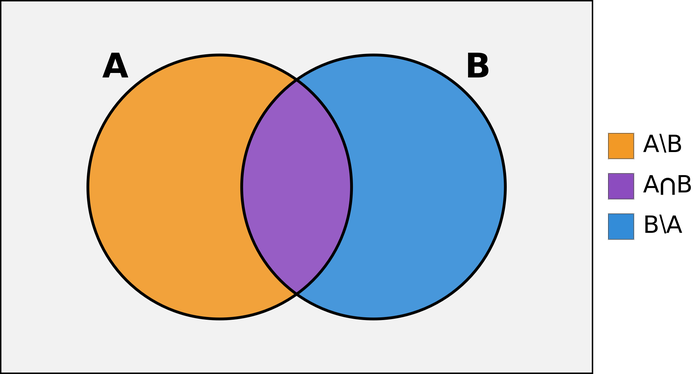
\includegraphics[width=0.75\linewidth]{imagenes/tema2/T2_1_a.png}
\end{center}
\begin{center}
    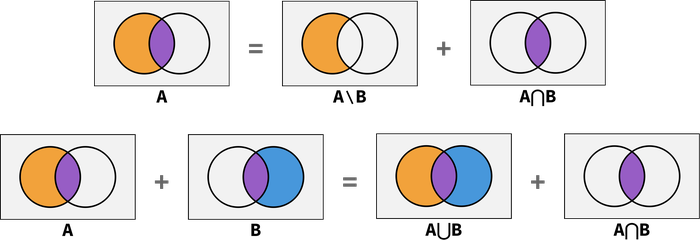
\includegraphics[width=0.75\linewidth]{imagenes/tema2/T2_1_b.png}
\end{center}
\begin{center}
    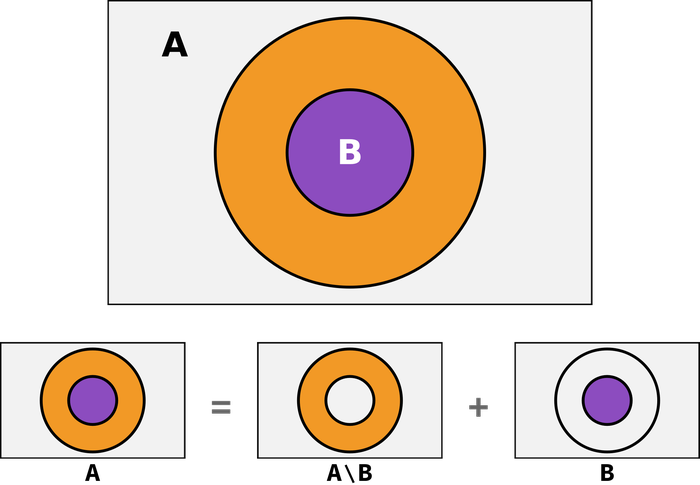
\includegraphics[width=0.75\linewidth]{imagenes/tema2/T2_1_c.png}
\end{center}
\begin{center}
    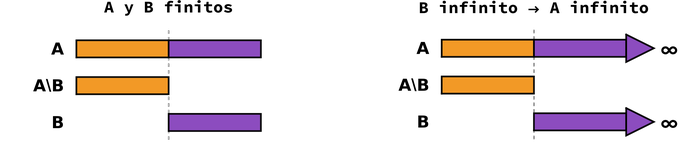
\includegraphics[width=0.75\linewidth]{imagenes/tema2/T2_1_d.png}
\end{center}
\end{demostracion}

\newpage
%=========================================================
%=== SECCIÓN 2. CONTINUIDAD DE FUNCIONES DE CONJUNTO =====
%=========================================================
\section{Continuidad de funciones de conjunto}

\begin{definicion}{Continuidad ascendente/descendente}{continuidad}
    Una función de conjunto $\mu$ se dice \textbf{continua ascendente} si para toda sucesión $\{A_n\}$ creciente:
    \[
    \lim(\mu(A_n))=\mu(\lim(A_n))
    \]
    Una función de conjunto $\mu$ se dice \textbf{continua descendendente} si para toda sucesión $\{A_n\}$ decreciente tal que $|\mu(A_{n_0}|<\infty$, para algún $n_0$, se verifica:
    \[
    \lim(\mu(A_n))=\mu(\lim(A_n))
    \]
    Estas definiciones tienen sentido cuando el dominio de definición de $\mu$ es una clase monótona. Como solo aplican a sucesiones monótonas de conjuntos, son siempre convergentes y el límite siempre existe.

    Diremos que $\mu$ es \textbf{continua} si lo es ascendente y descendentemente.

    Diremos que $\mu$ es \textbf{continua en un conjunto} $A$ si es continua para toda sucesión monótona que converja a $A$.
\end{definicion}

\begin{teorema}{Relación entre continuidad y \texorpdfstring{$\sigma$}{sigma}-aditividad}{teo4}
Sea $\mathcal{G}$ una $\sigma$-álgebra sobre $\Omega$ y $\mu : \mathcal{G} \to \overline{\mathbb{R}}$ una función de conjunto aditiva. Se verifican las siguientes propiedades:
\begin{enumerate}[label=\alph*)]
    \item Si $\mu$ es continua ascendente, entonces $\mu$ es $\sigma$-aditiva.
    \item Si $\mu$ es continua descendente en el vacío ($\varnothing$) y finita, entonces $\mu$ es $\sigma$-aditiva.
\end{enumerate}
\end{teorema}

\begin{demostracion}
Sea $\{A_n\}_{n \in \mathbb{N}} \subseteq \mathcal{G}$ una sucesión de conjuntos disjuntos dos a dos ($A_i \cap A_j = \varnothing$ para todo $i \neq j$).

\begin{enumerate}[label=\alph*)]
    \item Definimos la sucesión de uniones finitas parciales:
    \[
        C_n = \bigcup_{i=1}^n A_i
    \]
    Por construcción, $\{C_n\}_{n \in \mathbb{N}}$ es una sucesión monótona creciente ($C_n \uparrow$) cuyo límite es la unión numerable infinita:
    \[
        \lim_{n \to \infty} C_n = \bigcup_{n=1}^\infty C_n = \bigcup_{i=1}^\infty A_i
    \]
    
    Aplicando la hipótesis de continuidad ascendente de $\mu$ sobre la sucesión $\{C_n\}$ y la aditividad finita de $\mu$ sobre la unión disjunta $C_n = \bigcup_{i=1}^n A_i$:
    \begin{align*}
        \mu\left( \bigcup_{i=1}^\infty A_i \right) &= \mu\left( \lim_{n \to \infty} C_n \right) = \lim_{n \to \infty} \mu(C_n) \\
        &= \lim_{n \to \infty} \mu\left( \bigcup_{i=1}^n A_i \right) = \lim_{n \to \infty} \sum_{i=1}^n \mu(A_i) = \sum_{i=1}^\infty \mu(A_i)
    \end{align*}
    Por consiguiente, $\mu$ es $\sigma$-aditiva.

    \item Definimos la sucesión cola de la unión numerable:
     \[
     D_n = \displaystyle\left( \bigcup_{i=1}^\infty A_i \right) \setminus C_n
     \]
    
    Observamos que la sucesión $\{D_n\}_{n \in \mathbb{N}}$ es monótona decreciente ($D_n \downarrow$) y su límite viene dado por:
    \[
        \lim_{n \to \infty} D_n = \left( \bigcup_{i=1}^\infty A_i \right) \setminus \left( \lim_{n \to \infty} C_n \right) = \left( \bigcup_{i=1}^\infty A_i \right) \setminus \left( \bigcup_{i=1}^\infty A_i \right) = \varnothing
    \]
    
    Puesto que la función de conjunto $\mu$ es finita por hipótesis, se cumple $|\mu(D_n)| < \infty$ para todo $n \in \mathbb{N}$. Por tanto, podemos aplicar la propiedad de continuidad descendente en el vacío:
    \[
        \lim_{n \to \infty} \mu(D_n) = \mu\left( \lim_{n \to \infty} D_n \right) = \mu(\varnothing) = 0
    \]
    
    Por otra parte, para cada $n \in \mathbb{N}$, el conjunto total se descompone de forma disjunta como $\bigcup_{i=1}^\infty A_i = C_n \cup D_n$, con $C_n \cap D_n = \varnothing$. Usando la aditividad finita de $\mu$:
    \[
        \mu\left( \bigcup_{i=1}^\infty A_i \right) = \mu(C_n \cup D_n) = \mu(C_n) + \mu(D_n) = \sum_{i=1}^n \mu(A_i) + \mu(D_n)
    \]
    
    Tomando el límite cuando $n \to \infty$ en ambos lados y considerando que la cantidad $\mu\left( \bigcup_{i=1}^\infty A_i \right)$ es una constante respecto de $n$:
    \begin{align*}
        \mu\left( \bigcup_{i=1}^\infty A_i \right) &= \lim_{n \to \infty} \mu\left( \bigcup_{i=1}^\infty A_i \right) = \lim_{n \to \infty} \left( \sum_{i=1}^n \mu(A_i) + \mu(D_n) \right) \\
        &= \sum_{i=1}^\infty \mu(A_i) + \lim_{n \to \infty} \mu(D_n) = \sum_{i=1}^\infty \mu(A_i) + 0 = \sum_{i=1}^\infty \mu(A_i)
    \end{align*}
    Queda demostrado que $\mu$ es $\sigma$-aditiva.
\end{enumerate}

\begin{center}
    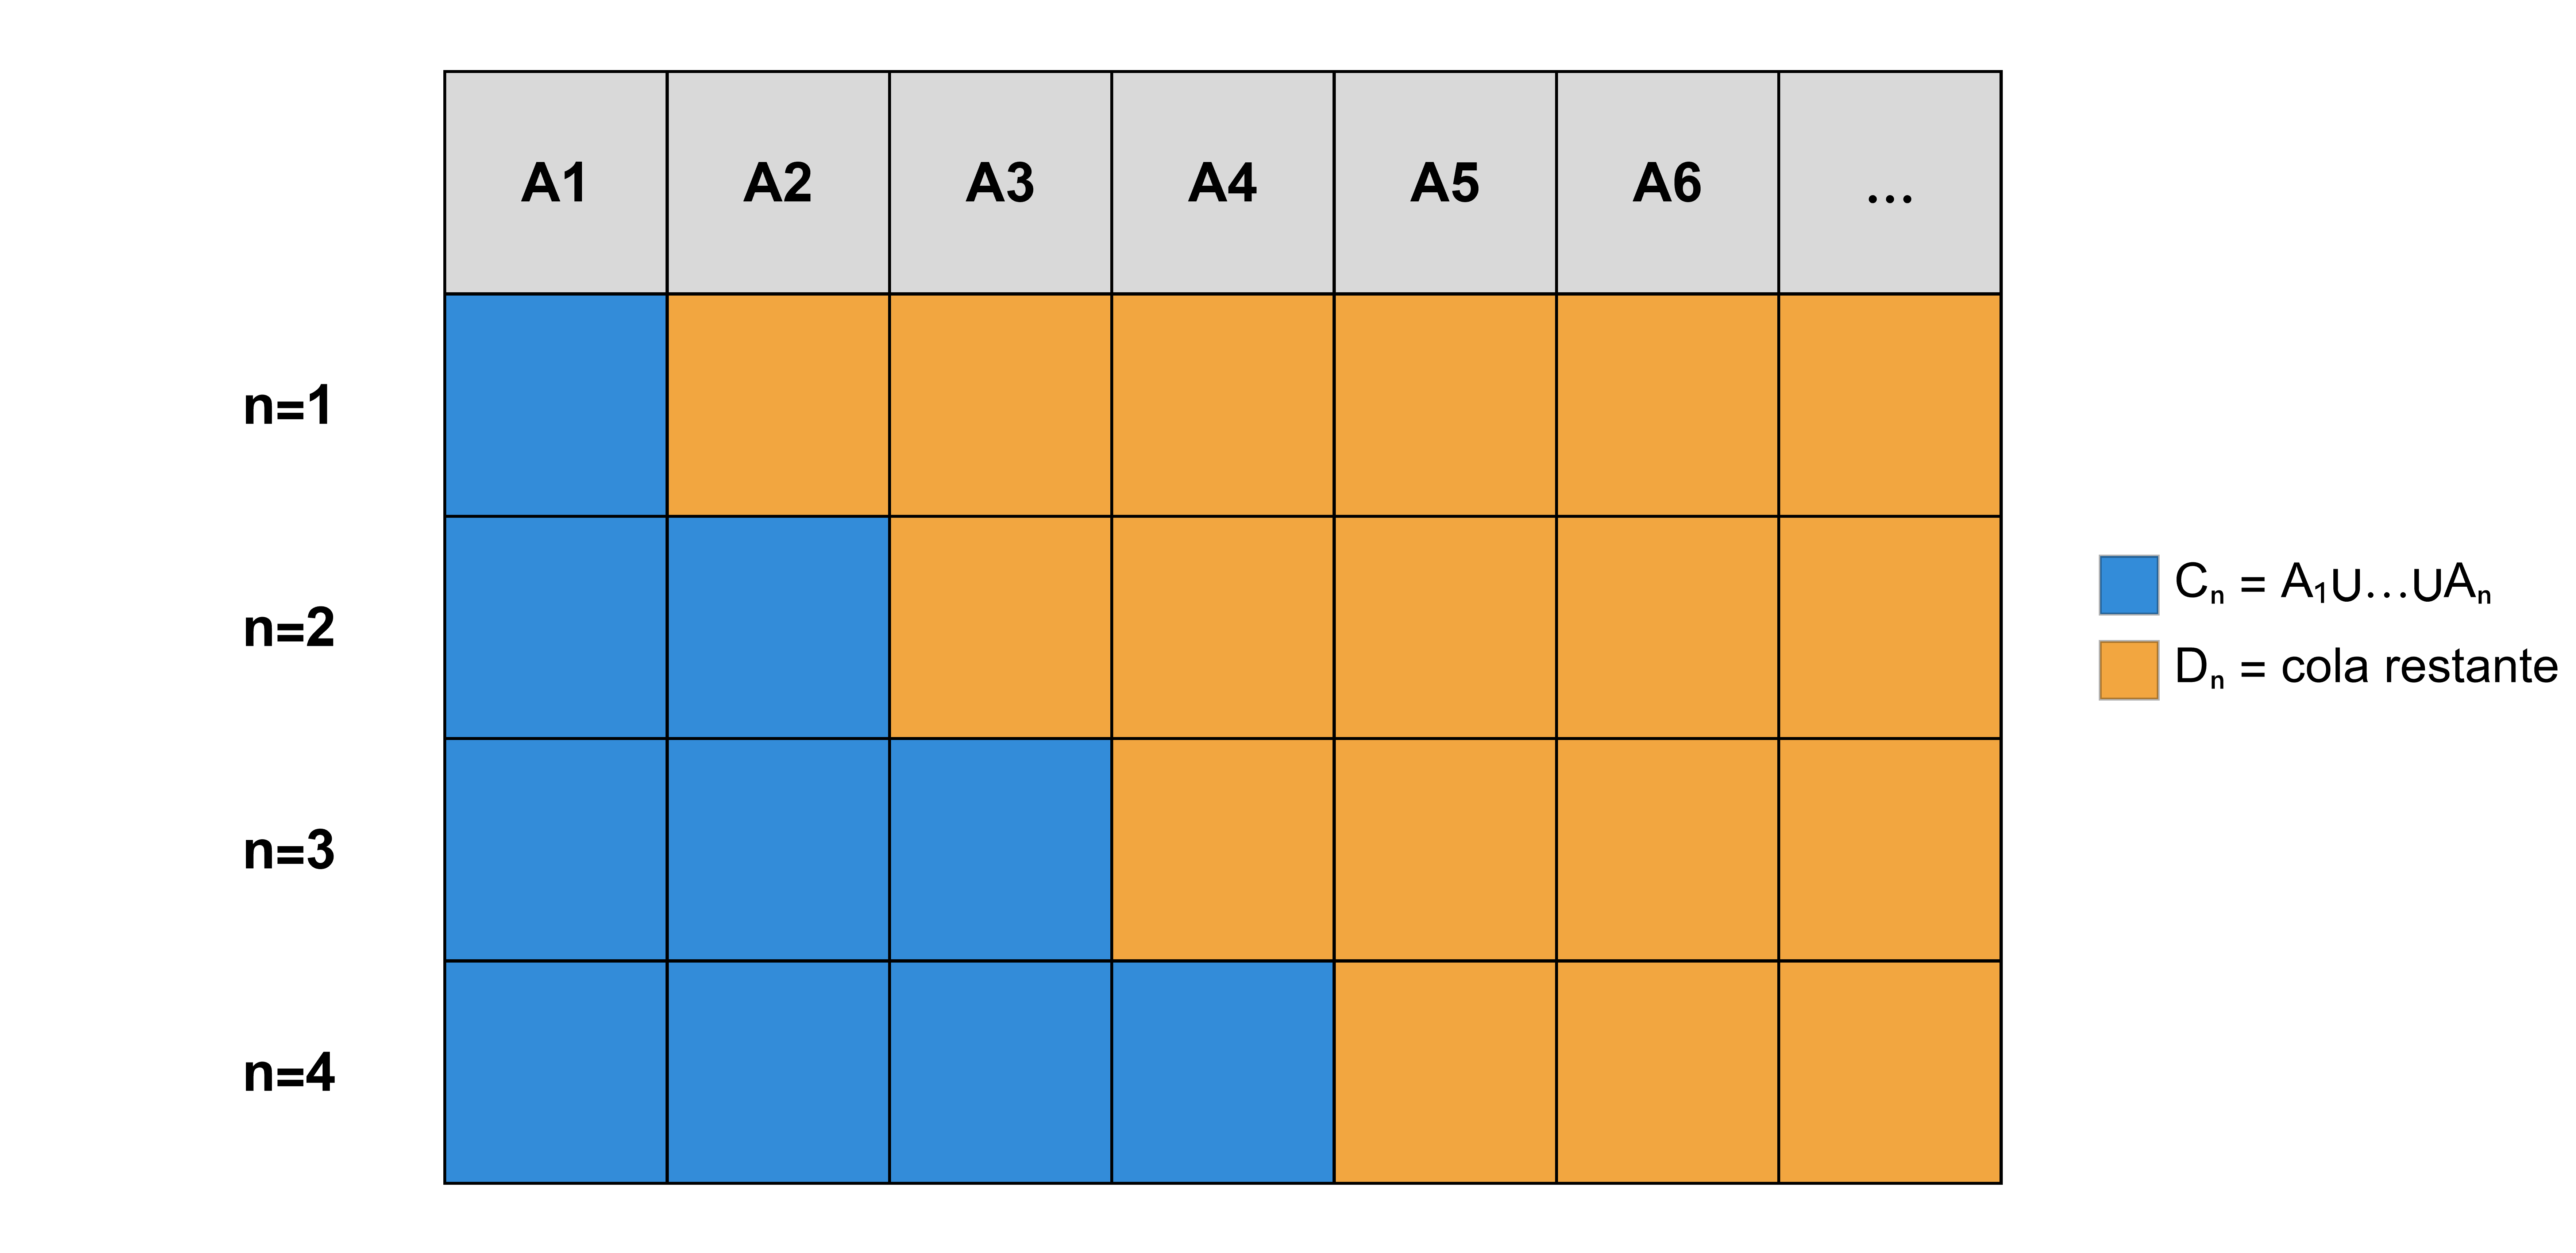
\includegraphics[width=0.75\linewidth]{imagenes/tema2/T2_1_teorema4.png}
\end{center}
\end{demostracion}

\newpage

\begin{teorema}{Teorema de continuidad}{teo5}
Sea $\mathcal{G}$ una $\sigma$-álgebra sobre $\Omega$ y $\mu : \mathcal{G} \to \overline{\mathbb{R}}$ una función de conjunto aditiva. Si $\mu$ es $\sigma$-aditiva, entonces $\mu$ es continua.
\end{teorema}

\begin{demostracion}
Para probar que $\mu$ es continua, debemos demostrar que es continua ascendente y continua descendente.

\begin{enumerate}[label=\arabic*.]
    \item \textbf{Continuidad ascendente:}
    
    Sea $\{A_n\}_{n \in \mathbb{N}} \subseteq \mathcal{G}$ una sucesión creciente de conjuntos ($A_1 \subseteq A_2 \subseteq \dots \subseteq A_n \subseteq \dots$). Su límite viene dado por $\displaystyle \lim_{n \to \infty} A_n = \bigcup_{i=1}^\infty A_i$. Distinguimos dos casos:
    
    \begin{itemize}
        \item \textit{Caso 1: Existe algún $k \in \mathbb{N}$ tal que $\mu(A_k) = \pm\infty$.}
        
        Por la propiedad 4 de las funciones de conjunto aditivas, al ser $A_k \subseteq A_n$ para todo $n \ge k$, se tiene que $\mu(A_n) = \pm\infty$ para todo $n \ge k$, de donde:
        \[
            \lim_{n \to \infty} \mu(A_n) = \pm\infty
        \]
        Análogamente, como $A_k \subseteq \bigcup_{i=1}^\infty A_i = \lim_{n \to \infty} A_n$, se verifica que:
        \[
            \mu\left( \lim_{n \to \infty} A_n \right) = \pm\infty
        \]
        Por tanto, en este caso se cumple trivialmente $\displaystyle \lim_{n \to \infty} \mu(A_n) = \mu\left( \lim_{n \to \infty} A_n \right) = \pm\infty$.

        \item \textit{Caso 2: $|\mu(A_n)| < +\infty$ para todo $n \in \mathbb{N}$.}
        
        Definimos la sucesión de conjuntos disjuntos $\{B_n\}_{n \in \mathbb{N}}$ mediante las coronas (tomando $A_0 = \varnothing$):
        \[
            B_n = A_n \setminus A_{n-1}, \quad \forall n \in \mathbb{N}
        \]
        Esta sucesión satisface las siguientes propiedades:
        \begin{itemize}
            \item $\displaystyle \bigcup_{i=1}^n B_i = A_n \quad \text{y} \quad \bigcup_{i=1}^\infty B_i = \bigcup_{i=1}^\infty A_i = \lim_{n \to \infty} A_n$.
            \item Por la propiedad 3, dado que $A_{n-1} \subseteq A_n$ y $\mu(A_{n-1})$ es finita:
            \[
                \mu(B_n) = \mu(A_n \setminus A_{n-1}) = \mu(A_n) - \mu(A_{n-1})
            \]
        \end{itemize}
        Dado que $\mu$ es $\sigma$-aditiva por hipótesis, calculamos la medida del límite:
        \begin{align*}
            \mu\left( \lim_{n \to \infty} A_n \right) &= \mu\left( \bigcup_{i=1}^\infty A_i \right) = \mu\left( \bigcup_{i=1}^\infty B_i \right) = \sum_{i=1}^\infty \mu(B_i) \\
            &= \lim_{n \to \infty} \sum_{i=1}^n \mu(B_i) = \lim_{n \to \infty} \sum_{i=1}^n \bigl[ \mu(A_i) - \mu(A_{i-1}) \bigr] \\
            &= \lim_{n \to \infty} \mu(A_n)
        \end{align*}
    \end{itemize}
    En ambos casos se verifica que $\displaystyle \lim_{n \to \infty} \mu(A_n) = \mu\left( \lim_{n \to \infty} A_n \right)$, demostrando que $\mu$ es continua ascendente.

    \item \textbf{Continuidad descendente:}
    
    Sea $\{A_n\}_{n \in \mathbb{N}} \subseteq \mathcal{G}$ una sucesión decreciente ($A_1 \supseteq A_2 \supseteq \dots \supseteq A_n \supseteq \dots$) tal que existe algún $k \in \mathbb{N}$ con $\mu(A_k)$ finito.
    
    Por la propiedad 5 de las funciones de conjunto aditivas:
    \begin{itemize}
        \item $\mu(A_n)$ es finita para todo $n \ge k$.
        \item Dado que $\displaystyle \lim_{n \to \infty} A_n = \bigcap_{i=1}^\infty A_i \subseteq A_k$, la medida $\displaystyle \mu\left( \lim_{n \to \infty} A_n \right)$ es también finita.
    \end{itemize}

    Fijando dicho conjunto $A_k$, definimos la sucesión auxiliar:
    \[
        B_n = A_k \setminus A_{n+k-1}, \quad \forall n \in \mathbb{N}
    \]
    Al ser $\{A_n\}$ decreciente, la sucesión $\{B_n\}$ es monótona creciente ($B_n \uparrow$), y su límite es:
    \[
        \lim_{n \to \infty} B_n = \lim_{n \to \infty} (A_k \setminus A_{n+k-1}) = A_k \setminus \left( \lim_{n \to \infty} A_n \right)
    \]

    Por la continuidad ascendente probada en el apartado anterior, se verifica que:
    \[
        \mu\left( \lim_{n \to \infty} B_n \right) = \lim_{n \to \infty} \mu(B_n)
    \]
    Desarrollamos ambos miembros de esta igualdad de forma independiente:
    \begin{itemize}
        \item \textit{Miembro izquierdo:} Aplicando la propiedad 3 (ya que $\displaystyle \lim_{n \to \infty} A_n \subseteq A_k$ y su medida es finita):
        \[
            \mu\left( \lim_{n \to \infty} B_n \right) = \mu\left( A_k \setminus \lim_{n \to \infty} A_n \right) = \mu(A_k) - \mu\left( \lim_{n \to \infty} A_n \right)
        \]
        \item \textit{Miembro derecho:} Puesto que $\mu(A_{n+k-1})$ es finita para todo $n \ge 1$:
        \begin{align*}
            \lim_{n \to \infty} \mu(B_n) &= \lim_{n \to \infty} \mu(A_k \setminus A_{n+k-1}) = \lim_{n \to \infty} \bigl[ \mu(A_k) - \mu(A_{n+k-1}) \bigr] \\
            &= \mu(A_k) - \lim_{n \to \infty} \mu(A_{n+k-1}) = \mu(A_k) - \lim_{n \to \infty} \mu(A_n)
        \end{align*}
    \end{itemize}

    Igualando ambas expresiones:
    \[
        \mu(A_k) - \mu\left( \lim_{n \to \infty} A_n \right) = \mu(A_k) - \lim_{n \to \infty} \mu(A_n)
    \]
    Al ser $\mu(A_k)$ una cantidad finita, restando $\mu(A_k)$ en ambos lados se concluye:
    \[
        \lim_{n \to \infty} \mu(A_n) = \mu\left( \lim_{n \to \infty} A_n \right)
    \]
    lo que prueba que $\mu$ es continua descendente.
\end{enumerate}

Al ser continua tanto ascendente como descendentemente, queda demostrado que la función de conjunto $\mu$ es continua.

\begin{center}
    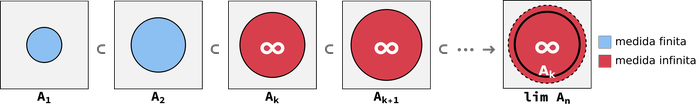
\includegraphics[width=0.75\linewidth]{imagenes/tema2/T2_1_e.png}
\end{center}
\begin{center}
    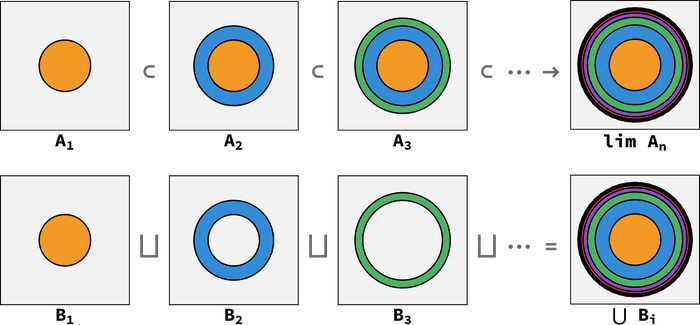
\includegraphics[width=0.75\linewidth]{imagenes/tema2/T2_1_f.png}
\end{center}
\begin{center}
    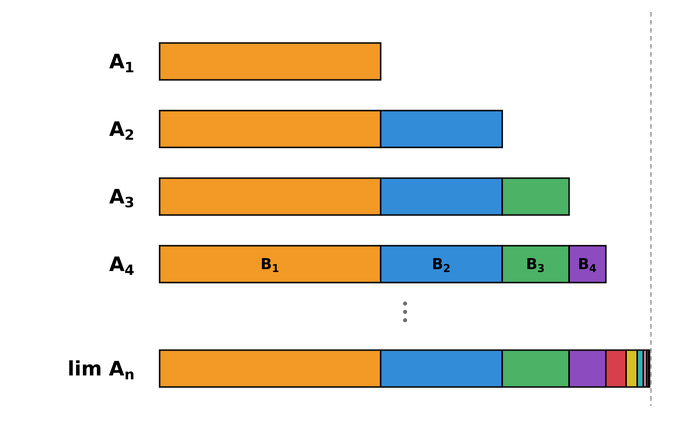
\includegraphics[width=0.75\linewidth]{imagenes/tema2/T2_1_g.png}
\end{center}
\begin{center}
    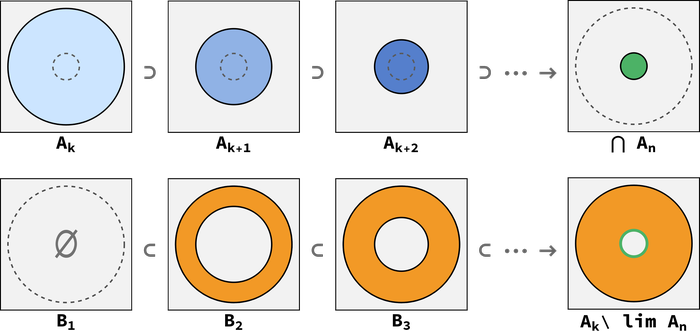
\includegraphics[width=0.75\linewidth]{imagenes/tema2/T2_1_h.png}
\end{center}
\end{demostracion}

\newpage
%=========================================================
%================= SECCIÓN 3. MEDIDAS ====================
%=========================================================
\section{Medidas}
\begin{definicion}{Medida y espacio medible}{medidas}
    Llamaremos \textbf{medida} a una función de conjunto $\sigma$-aditiva y positiva.

    Dado un conjunto universal $\Omega$ y una $\sigma$-álgebra $\mathcal{G}$ de subconjuntos de $\Omega$, al par $(\Omega, \mathcal{G})$ se le denomina \textbf{espacio medible}, y a los elementos de $\mathcal{G}$ se les llama \textbf{conjuntos medibles}.

    Sea $\mu : \mathcal{G} \to \overline{\mathbb{R}}$ una medida. A la terna $(\Omega, \mathcal{G}, \mu)$ se le denomina \textbf{espacio de medida}. 

    Si además $\mu(\Omega) = 1$, decimos que $\mu$ es una \textbf{probabilidad} o \textbf{medida probabilística}, y a la terna $(\Omega, \mathcal{G}, \mu)$ se le llama \textbf{espacio probabilístico} o \textbf{espacio de probabilidad}.

\end{definicion}

\begin{proposicion}{Propiedades básicas de las medidas}{prop:prop11}
Para toda medida $\mu : \mathcal{G} \to \overline{\mathbb{R}}$ se verifican las siguientes propiedades:
\begin{enumerate}[label=\alph*)]
    \item \textbf{Monotonía:} Si $A, B \in \mathcal{G}$ con $B \subseteq A$, entonces $\mu(B) \le \mu(A)$.
    \item \textbf{Subaditividad numerable:} Para toda sucesión de conjuntos $\{A_n\}_{n \in \mathbb{N}} \subseteq \mathcal{G}$, se satisface:
    \[
        \mu\left( \bigcup_{n=1}^\infty A_n \right) \le \sum_{n=1}^\infty \mu(A_n)
    \]
\end{enumerate}
\end{proposicion}

\begin{demostracion}
Al ser una medida una función de conjunto $\sigma$-aditiva y positiva, satisface en particular todas las propiedades de las funciones aditivas:

\begin{enumerate}[label=\alph*)]
    \item Por la propiedad de aditividad, podemos descomponer $A$ como la unión disjunta $A = (A \setminus B) \cup B$. Por consiguiente:
    \[
        \mu(A) = \mu(A \setminus B) + \mu(B)
    \]
    Como $\mu$ es una función de conjunto positiva, se tiene que $\mu(A \setminus B) \ge 0$, de lo cual se deduce directamente que $\mu(A) \ge \mu(B)$.

    \item Sean $A_1, A_2 \in \mathcal{G}$. Aplicando la propiedad aditiva general:
    \[
        \mu(A_1) + \mu(A_2) = \mu(A_1 \cup A_2) + \mu(A_1 \cap A_2)
    \]
    Dado que $\mu(A_1 \cap A_2) \ge 0$, se obtiene $\mu(A_1 \cup A_2) \le \mu(A_1) + \mu(A_2)$.
    
    Por inducción finita, para cualquier número $n$ de subconjuntos se verifica:
    \[
        \mu\left( \bigcup_{j=1}^n A_j \right) \le \sum_{j=1}^n \mu(A_j)
    \]
    Tomando el límite cuando $n \to \infty$ en ambos miembros de la desigualdad:
    \[
        \lim_{n \to \infty} \mu\left( \bigcup_{j=1}^n A_j \right) \le \lim_{n \to \infty} \sum_{j=1}^n \mu(A_j) = \sum_{n=1}^\infty \mu(A_n)
    \]
    Por otra parte, la sucesión de uniones finitas $B_n = \bigcup_{j=1}^n A_j$ es una sucesión monótona creciente ($B_n \uparrow$) cuyo límite es la unión numerable infinita:
    \[
        \lim_{n \to \infty} B_n = \bigcup_{n=1}^\infty A_n
    \]
    Dado que toda medida $\sigma$-aditiva es continua ascendente, podemos conmutar el límite con la medida:
    \[
        \lim_{n \to \infty} \mu\left( \bigcup_{j=1}^n A_j \right) = \lim_{n \to \infty} \mu(B_n) = \mu\left( \lim_{n \to \infty} B_n \right) = \mu\left( \bigcup_{n=1}^\infty A_n \right)
    \]
    Sustituyendo este resultado en la desigualdad anterior se obtiene la propiedad de subaditividad numerable.
\end{enumerate}
\end{demostracion}
\noindent
\textbf{Nota previa: Repaso de límites de sucesiones numéricas}\\
Para estudiar cuándo es posible conmutar la medida con el límite para sucesiones de conjuntos no necesariamente monótonas, recordamos las definiciones y propiedades fundamentales de los límites superior e inferior de sucesiones reales.

Dada una sucesión numérica $\{a_n\}_{n \in \mathbb{N}} \subseteq \overline{\mathbb{R}}$, sus límites superior e inferior se definen como:
\[
    \varlimsup_{n \to \infty} a_n = \limsup_{n \to \infty} a_n \equiv \inf_{n \ge 1} \sup_{m \ge n} a_m
\]
\[
    \varliminf_{n \to \infty} a_n = \liminf_{n \to \infty} a_n \equiv \sup_{n \ge 1} \inf_{m \ge n} a_m
\]
\begin{itemize}
    \item Los límites superior e inferior siempre existen en $\overline{\mathbb{R}}$.
    \item Se verifica siempre la relación $\displaystyle \varliminf_{n \to \infty} a_n \le \varlimsup_{n \to \infty} a_n$.
    \item Si ambos coinciden, la sucesión $\{a_n\}$ es convergente y $\displaystyle \lim_{n \to \infty} a_n = \varliminf_{n \to \infty} a_n = \varlimsup_{n \to \infty} a_n$.
    \item Si $\{a_n\}$ es monótona creciente (resp. decreciente), es convergente a su supremo (resp. ínfimo).
    \item Si $\{a_n\}$ y $\{b_n\}$ son sucesiones tales que $a_n \le b_n$ para todo $n \in \mathbb{N}$, se cumple:
    \[
        \varliminf_{n \to \infty} a_n \le \varliminf_{n \to \infty} b_n \quad \text{y} \quad \varlimsup_{n \to \infty} a_n \le \varlimsup_{n \to \infty} b_n
    \]
\end{itemize}

\newpage

\begin{teorema}{Teorema de continuidad para medidas}{teo6}
Sea $\mu : \mathcal{G} \to \overline{\mathbb{R}}$ una medida y sea $\{A_n\}_{n \in \mathbb{N}} \subseteq \mathcal{G}$ una sucesión arbitraria de conjuntos medibles. Se verifican las siguientes afirmaciones:
\begin{enumerate}[label=\alph*)]
    \item $\displaystyle \mu\left( \varliminf_{n \to \infty} A_n \right) \le \varliminf_{n \to \infty} \mu(A_n) \le \varlimsup_{n \to \infty} \mu(A_n)$
    \item Si existe un índice $n_0 \in \mathbb{N}$ tal que $\displaystyle \mu\left( \bigcup_{j=n_0}^\infty A_j \right) < \infty$, entonces:
    \[
        \mu\left( \varliminf_{n \to \infty} A_n \right) \le \varliminf_{n \to \infty} \mu(A_n) \le \varlimsup_{n \to \infty} \mu(A_n) \le \mu\left( \varlimsup_{n \to \infty} A_n \right)
    \]
    \item Si además la sucesión de conjuntos $\{A_n\}$ es convergente, entonces la sucesión numérica $\{\mu(A_n)\}$ es convergente y se cumple:
    \[
        \mu\left( \lim_{n \to \infty} A_n \right) = \lim_{n \to \infty} \mu(A_n)
    \]
\end{enumerate}
\end{teorema}

\begin{demostracion}
\begin{enumerate}[label=\alph*)]
    \item Consideremos la sucesión de conjuntos $\delta_n = \bigcap_{j=n}^\infty A_j$. Se cumple que:
    \begin{itemize}
        \item[i)] $\{\delta_n\}_{n \in \mathbb{N}}$ es una sucesión monótona creciente, luego tiene límite y es
        \[
            \lim_{n \to \infty} \delta_n = \bigcup_{n=1}^\infty \bigcap_{j=n}^\infty A_j = \varliminf_{n \to \infty} A_n
        \]
        \item[ii)] Como toda medida es continua ascendente:
        \[
             \mu\left( \lim_{n \to \infty} \delta_n \right) = \lim_{n \to \infty} \mu(\delta_n)
        \]
        \item[iii)] La sucesión numérica $\{\mu(\delta_n)\}$ es creciente y por tanto convergente. Además, como $\delta_n \subseteq A_n$ para todo $n \in \mathbb{N}$, por monotonía de la medida se tiene 
        \[
            \mu(\delta_n) \le \mu(A_n) \:\implies\:\varliminf_{n \to \infty} \mu(\delta_n) \le \varliminf_{n \to \infty} \mu(A_n)
        \]
    \end{itemize}
    Por consiguiente,
    \[
    \mu(\varliminf_{n \to \infty} A_n) \overset{i)}{=} \mu(\lim_{n \to \infty}\delta_n) \overset{ii)}{=} \lim_{n \to \infty}\mu(\delta_n)=\varliminf_{n \to \infty}\mu(\delta_n) \overset{iii)}{\leq} \varliminf_{n \to \infty}\mu(A_n)
    \]
    La segunda desigualdad $\displaystyle \varliminf_{n \to \infty} \mu(A_n) \le \varlimsup_{n \to \infty} \mu(A_n)$ es una propiedad general para cualquier sucesión numérica.
\newpage
    \item Falta demostrar la tercera desigualdad, para ello consideramos la sucesión de conjuntos $\sigma_n = \bigcup_{j=n}^\infty A_j$. La sucesión $\{\sigma_n\}_{n \in \mathbb{N}}$ es monótona decreciente ($\sigma_n \downarrow$) y su límite es el límite superior de la sucesión:
    \begin{itemize}
        \item[i)] $\{\sigma_n\}_{n \in \mathbb{N}}$ es una sucesión monótona decreciente, luego tiene límite y es
        \[
            \lim_{n \to \infty} \sigma_n = \bigcap_{n=1}^\infty \bigcup_{j=n}^\infty A_j = \varlimsup_{n \to \infty} A_n
        \]
        \item[ii)] Por hipótesis, existe $n_0 \in \mathbb{N}$ tal que $\mu(\sigma_{n_0}) < \infty$. Por el Teorema de continuidad, la medida $\mu$ es continua descendente sobre la sucesión $\{\sigma_n\}$:
        \[
            \mu\left( \lim_{n \to \infty} \sigma_n \right) = \lim_{n \to \infty} \mu(\sigma_n)
        \]
        \item[iii)] La sucesión numérica $\{\mu(\sigma_n)\}$ es decreciente y por tanto convergente. Además, como $A_n \subseteq \sigma_n$ para todo $n \in \mathbb{N}$, por monotonía de la medida se tiene 
        \[
            \mu(A_n) \le \mu(\sigma_n) \:\implies\:\varlimsup_{n \to \infty} \mu(A_n) \le \varlimsup_{n \to \infty} \mu(\sigma_n)
        \]
    \end{itemize}
    Por consiguiente,
    \[
    \varlimsup\mu(\sigma_n)=\varlimsup
    \]
    \[
        \varlimsup_{n \to \infty} \mu(A_n) \overset{iii)}{\le} \varlimsup_{n \to \infty} \mu(\sigma_n)  = \lim_{n \to \infty} \mu(\sigma_n) \overset{ii)}{=} \mu\left(\lim_{n\to\infty}\sigma_n\right) \overset{i)}{=} \mu\left( \varlimsup_{n \to \infty} A_n \right)
    \]


    \item Si la sucesión $\{A_n\}$ es convergente, sus límites superior e inferior de conjuntos coinciden:
    \[
        \varliminf_{n \to \infty} A_n = \varlimsup_{n \to \infty} A_n = \lim_{n \to \infty} A_n
    \]
    Sustituyendo esta igualdad en la cadena de desigualdades obtenida en el apartado b), los extremos de la cadena se igualan:
    \[
        \mu\left( \lim_{n \to \infty} A_n \right) \le \varliminf_{n \to \infty} \mu(A_n) \le \varlimsup_{n \to \infty} \mu(A_n) \le \mu\left( \lim_{n \to \infty} A_n \right)
    \]
    Por el teorema del sándwich, todas las desigualdades se convierten en igualdades. En particular, $\displaystyle \varliminf_{n \to \infty} \mu(A_n) = \varlimsup_{n \to \infty} \mu(A_n)$, lo que prueba que el límite numérico $\displaystyle \lim_{n \to \infty} \mu(A_n)$ existe y satisface $\displaystyle \mu\left( \lim_{n \to \infty} A_n \right) = \lim_{n \to \infty} \mu(A_n)$.
\end{enumerate}
\end{demostracion}

\begin{corolario}{Continuidad para medidas de probabilidad}{cor1}
Si $P : \mathcal{G} \to \mathbb{R}$ es una medida de probabilidad y $\{A_n\}_{n \in \mathbb{N}}$ es una sucesión arbitraria de sucesos de $\mathcal{G}$, se verifica:
\begin{enumerate}[label=\alph*)]
    \item $\displaystyle P\left( \varliminf_{n \to \infty} A_n \right) \le \varliminf_{n \to \infty} P(A_n) \le \varlimsup_{n \to \infty} P(A_n) \le P\left( \varlimsup_{n \to \infty} A_n \right)$
    \item Si la sucesión $\{A_n\}$ es convergente, entonces $\displaystyle P\left( \lim_{n \to \infty} A_n \right) = \lim_{n \to \infty} P(A_n)$.
\end{enumerate}
\end{corolario}

\begin{definicion}{Tipos de medidas}{tipos_medidas}
    \begin{itemize}
        \item \textbf{Medida finita e infinita:} Una medida $\mu$ se dice \textit{finita} si $\mu(\Omega) < \infty$. Toda medida finita puede convertirse en una medida de probabilidad equivalente definiendo $\mu' = \frac{\mu}{\mu(\Omega)}$.
        \item \textbf{Medida $\sigma$-finita:} Decimos que un espacio de medida $(\Omega, \mathcal{G}, \mu)$ es \textit{$\sigma$-finito} si existe una sucesión de conjuntos medibles $\{A_n\}_{n \in \mathbb{N}} \subseteq \mathcal{G}$ tal que $\mu(A_n) < \infty$ para todo $n \in \mathbb{N}$ y que constituye un recubrimiento de $\Omega$ ($\bigcup_{n=1}^\infty A_n = \Omega$). Típicamente se considera una sucesión creciente hacia el universo ($A_n \uparrow \Omega$).
        
        \textit{Ejemplo:} El espacio de Lebesgue $(\mathbb{R}, \mathcal{B}, \lambda)$ es $\sigma$-finito, ya que la sucesión de intervalos $A_n = (-n, n)$ recubre $\mathbb{R}$ y cumple $\lambda((-n, n)) = 2n < \infty$.
        
        \item \textbf{Propiedad casi seguro (c.s.):} Una propiedad se verifica \textit{casi seguro} (c.s.) o \textit{casi en todas partes} respecto a $\mu$ si se cumple en todos los elementos de $\Omega$ salvo en un conjunto de medida nula, es decir, existe $A \in \mathcal{G}$ con $\mu(A^c) = 0$ tal que la propiedad se verifica para todo $\omega \in A$.
        
        \item \textbf{Medida completa:} Una medida $\mu$ es \textit{completa} sobre $\mathcal{G}$ si todo subconjunto de un conjunto de medida nula pertenece a $\mathcal{G}$ (y por tanto tiene medida nula). En tal caso, el espacio de medida $(\Omega, \mathcal{G}, \mu)$ se denomina \textit{espacio completo}.
    \end{itemize}
\end{definicion}

\newpage
%==========================================================
%========== SECCIÓN 4. COMPARACIÓN DE MEDIDAS =============
%==========================================================
\section{Comparación de medidas}

Sean $\mu, \nu : \mathcal{G} \to \overline{\mathbb{R}}$ dos funciones de conjunto $\sigma$-aditivas sobre el espacio medible $(\Omega, \mathcal{G})$.

\begin{definicion}{Medidas mutuamente singulares}{def:singulares}
Decimos que las medidas $\mu$ y $\nu$ son \textit{mutuamente singulares} (o ortogonales), y lo denotamos por $\nu \perp \mu$, si existe algún conjunto medible $A \in \mathcal{G}$ tal que:
\[
    \nu(A) = 0 \quad \text{y} \quad \mu(A^c) = 0
\]
En este caso, la medida $\nu$ está concentrada en el conjunto $A^c$, mientras que la medida $\mu$ está concentrada en el conjunto $A$.
\end{definicion}

\begin{definicion}{Continuidad absoluta de medidas}{def:abs_continua}
Decimos que $\nu$ es \textit{absolutamente continua} respecto a $\mu$, y lo denotamos por $\nu \ll \mu$, si y solo si $\nu$ se anula sobre todos los conjuntos de la $\sigma$-álgebra $\mathcal{G}$ sobre los que $\mu$ se anula. Es decir:
\[
    \forall A \in \mathcal{G}, \quad \mu(A) = 0 \implies \nu(A) = 0
\]
\end{definicion}

\begin{observacion}
La relación de continuidad absoluta $\ll$ define una relación de \textit{preorden} (reflexiva y transitiva) en el conjunto de todas las medidas sobre el espacio medible $(\Omega, \mathcal{G})$:
\begin{enumerate}[label=\arabic*.]
    \item \textbf{Reflexividad:} $\mu \ll \mu$ para toda medida $\mu$.
    \item \textbf{Transitividad:} Si $\nu_1 \ll \nu_2$ y $\nu_2 \ll \nu_3$, entonces $\nu_1 \ll \nu_3$.
\end{enumerate}
En general, la relación no es antisimétrica. Cuando dos medidas cumplen simultáneamente $\nu \ll \mu$ y $\mu \ll \nu$, se dice que $\mu$ y $\nu$ son \textit{medidas equivalentes} ($\mu \sim \nu$), lo que significa que comparten exactamente los mismos conjuntos de medida nula.
\end{observacion}

\begin{figure}[h]
    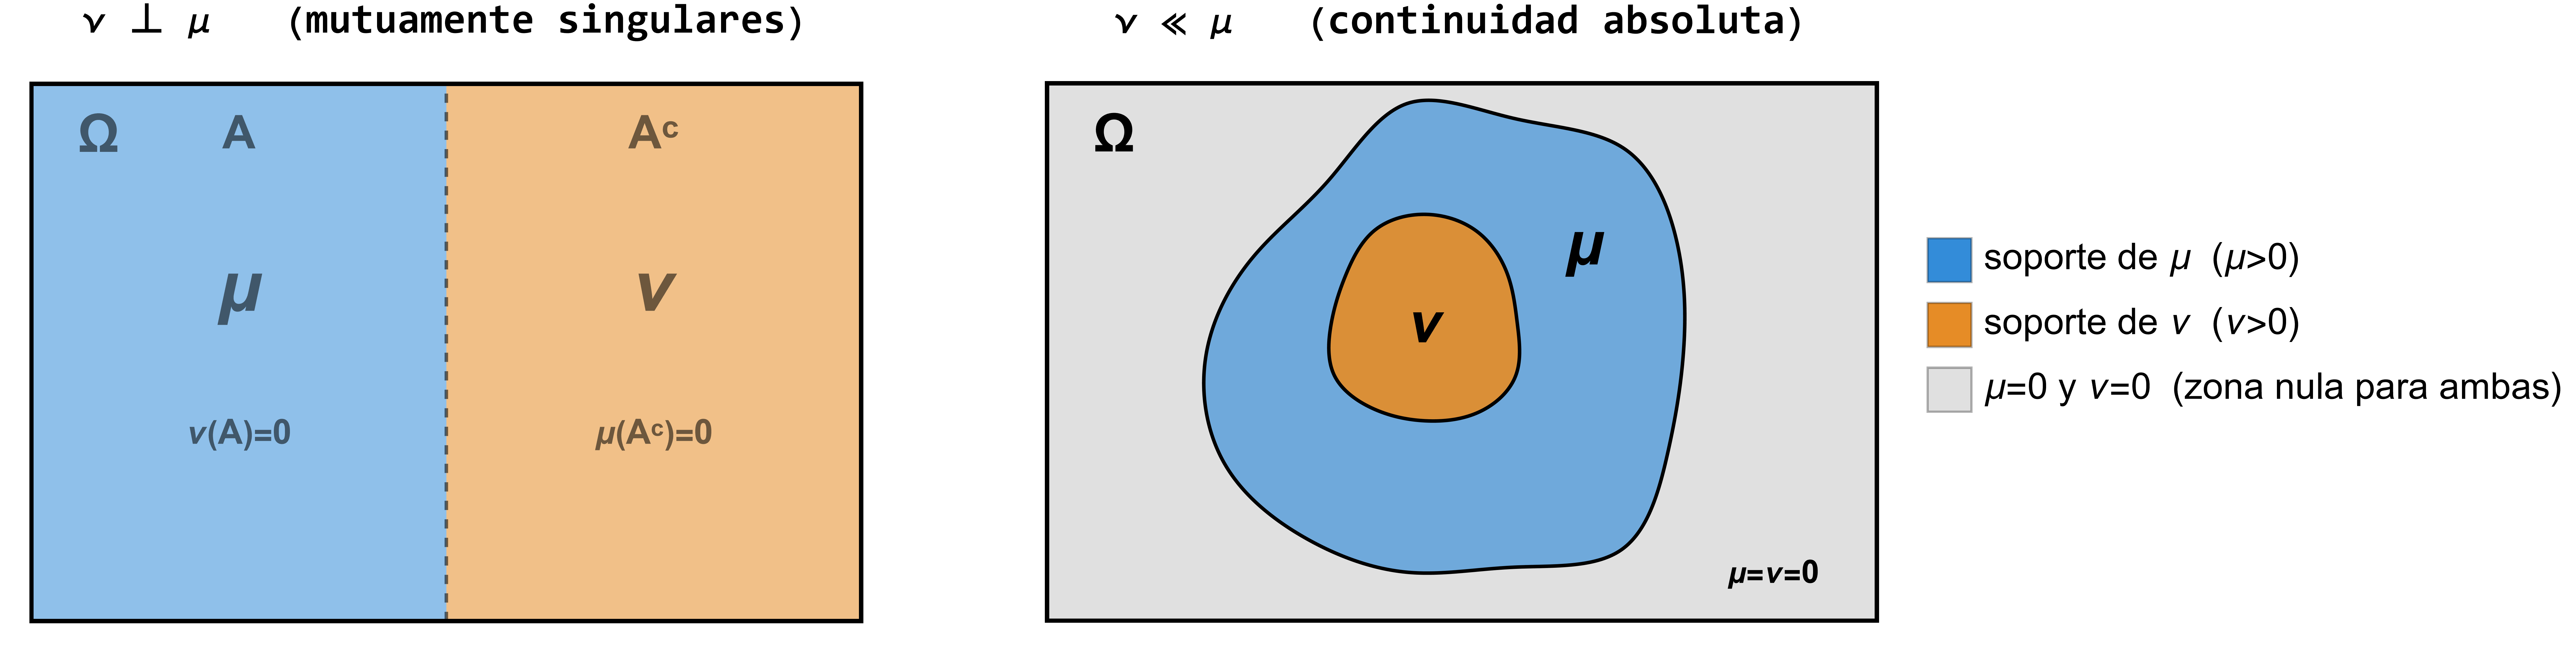
\includegraphics[width=0.95\textwidth]{imagenes/tema2/T2_2_comparacion_medidas.png}
\end{figure}

\begin{teorema}{Teorema de descomposición de Lebesgue}{teo:descomposicion_lebesgue}
Sean $\mu$ y $\nu$ dos medidas $\sigma$-finitas sobre el espacio medible $(\Omega, \mathcal{G})$. Entonces existe una única descomposición de la medida $\nu$ en la forma:
\[
    \nu = \nu_1 + \nu_2
\]
donde $\nu_1$ y $\nu_2$ son medidas $\sigma$-finitas sobre $\mathcal{G}$ tales que:
\[
    \nu_1 \perp \mu \quad \text{y} \quad \nu_2 \ll \mu
\]
\end{teorema}

\begin{demostracion}
\textbf{Comentarios sobre la estructura de la demostración:}
La componente $\nu_1$ representa la \textit{parte singular} de $\nu$ respecto de $\mu$, mientras que $\nu_2$ constituye la \textit{parte absolutamente continua} respecto de $\mu$. 

\begin{enumerate}[label=\arabic*.]
    \item \textbf{Existencia:} Se define la medida suma $\lambda = \mu + \nu$, la cual es también $\sigma$-finita sobre $\mathcal{G}$. Tanto $\mu$ como $\nu$ son absolutamente continuas respecto a $\lambda$ ($\mu \ll \lambda$ y $\nu \ll \lambda$). Mediante el Teorema de Radon-Nikodym, existen derivadas no negativas $f = \frac{d\mu}{d\lambda}$ y $g = \frac{d\nu}{d\lambda}$. Tomando el conjunto medible $A = \{\omega \in \Omega \mid f(\omega) = 0\}$, la restricción de $\nu$ al conjunto $A$ proporciona la componente singular $\nu_1(E) = \nu(E \cap A)$, mientras que la restricción al complementario $A^c$ genera la componente absolutamente continua $\nu_2(E) = \nu(E \cap A^c)$.
    
    \item \textbf{Unicidad:} Si existiera otra descomposición $\nu = \nu_1' + \nu_2'$ con $\nu_1' \perp \mu$ y $\nu_2' \ll \mu$, se obtendría $\nu_1 - \nu_1' = \nu_2' - \nu_2$. Al ser el miembro izquierdo una medida singular respecto a $\mu$ y el miembro derecho una medida absolutamente continua respecto a $\mu$, la única medida que satisface ambas condiciones simultáneamente es la medida nula, deduciéndose $\nu_1 = \nu_1'$ y $\nu_2 = \nu_2'$.
\end{enumerate}
\end{demostracion}

\newpage
%==========================================================
%========== SECCIÓN 5. EXTENSIÓN DE MEDIDAS ===============
%==========================================================
\section{Extensión de medidas}

En muchas aplicaciones prácticas (como en la construcción de la medida de Lebesgue en $\mathbb{R}^n$), resulta sencillo definir una medida sobre una clase de conjuntos simple (como rectángulos o intervalos) que forma una semialgebra, pero resulta necesario extenderla de forma coherente a estructuras más complejas como álgebras y $\sigma$-álgebras.

\begin{definicion}{Medida sobre una semialgebra}{def:medida_semialgebra}
Sea $S$ una semialgebra sobre un conjunto $\Omega$. Decimos que una función de conjunto $\mu : S \to \overline{\mathbb{R}}$ es una \textit{medida sobre la semialgebra} $S$ si satisface las siguientes condiciones:
\begin{enumerate}[label=\alph*)]
    \item \textbf{No negatividad:} $\mu(A) \ge 0$ para todo $A \in S$.
    \item \textbf{Conjunto vacío:} $\mu(\varnothing) = 0$.
    \item \textbf{$\sigma$-aditividad restringida:} Si $(A_n)_{n \in \mathbb{N}} \subseteq S$ es una sucesión de conjuntos disjuntos dos a dos tal que su unión numerable también pertenece a la semialgebra ($\bigcup_{n=1}^\infty A_n \in S$), entonces:
    \[
        \mu\left( \bigsqcup_{n=1}^\infty A_n \right) = \sum_{n=1}^\infty \mu(A_n)
    \]
\end{enumerate}
\end{definicion}

\begin{center}
    \vspace{0.2cm}
    \framebox[\linewidth]{\vbox to 2.2cm{\vfill \centering \textit{[Espacio reservado para diagrama: Esquema del proceso de extensión de medidas desde una semialgebra $S$ hasta la $\sigma$-álgebra $\sigma(S)$]} \vfill}}
    \vspace{0.2cm}
\end{center}

El proceso de extensión se realiza formalmente en dos etapas consecutivas:

\begin{teorema}{Primer teorema de extensión}{teo:primer_extension}
Sea $\mu$ una medida definida sobre una semialgebra $S$. Existe una única extensión $\bar{\mu}$ de la medida $\mu$ al álgebra generada por $S$, denotada por $\mathcal{Q}(S)$.
\end{teorema}

\begin{observacion}
Recordemos que todo elemento $E \in \mathcal{Q}(S)$ se expresa de forma única como una unión finita de elementos disjuntos de $S$ ($E = \bigsqcup_{i=1}^r A_i$ con $A_i \in S$). La extensión $\bar{\mu}$ en el álgebra se define de forma natural como $\bar{\mu}(E) = \sum_{i=1}^r \mu(A_i)$.
\end{observacion}

\begin{teorema}{Teorema de existencia y unicidad de Carathéodory}{teo:caratheodory}
Toda medida $\mu$ definida sobre un álgebra $\mathcal{Q}$ se extiende como una medida $\bar{\mu}$ a la $\sigma$-álgebra generada por $\mathcal{Q}$, denotada por $\sigma(\mathcal{Q})$.

Además, si la medida original $\mu$ es $\sigma$-finita sobre $\mathcal{Q}$, entonces su extensión $\bar{\mu}$ a $\sigma(\mathcal{Q})$ es \textbf{única} y también es \textbf{$\sigma$-finita}.
\end{teorema}

\begin{observacion}
El Teorema de Carathéodory es fundamental para garantizar la existencia de la medida de Lebesgue $\lambda$ en $\mathbb{R}^n$, partiendo de la medida del volumen elemental definida sobre los intervalos o rectángulos de $\mathbb{R}^n$. La condición de $\sigma$-finitud resulta indispensable para garantizar que no existan múltiples extensiones distintas sobre la misma $\sigma$-álgebra.
\end{observacion}

\newpage
%==========================================================
\seccionproblemas

% ------------------------------------------------------------------------------
% PROBLEMA 25
% ------------------------------------------------------------------------------
\begin{problema}[Aditividad y no $\sigma$-aditividad de la densidad natural relativa]
En el espacio medible $(\mathbb{N}, \mathcal{P}(\mathbb{N}))$, se definen para cada subconjunto de números naturales $E \subseteq \mathbb{N}$ las siguientes funciones de conjunto:
\[
    r_n(E) = \#\{k \in E \mid k \le n\}, \quad \tau(E) = \lim_{n \to \infty} \frac{r_n(E)}{n}
\]
Sea $\mathcal{G} = \{ E \subseteq \mathbb{N} \mid \text{existe el límite } \tau(E) \}$. Demostrar que la función de conjunto $\tau$ es aditiva sobre la clase $\mathcal{G}$, pero no es $\sigma$-aditiva.

\tcblower

\paragraph{1. Demostración de la aditividad sobre $\mathcal{G}$:}

Verificamos en primer lugar que $\tau$ cumple las condiciones de función de conjunto aditiva sobre la clase $\mathcal{G}$:
\begin{enumerate}[label=\alph*)]
    \item \textit{Pertenencia del conjunto vacío:} Para $E = \varnothing$, se tiene $r_n(\varnothing) = 0$ para todo $n \in \mathbb{N}$. Por tanto:
    \[
        \tau(\varnothing) = \lim_{n \to \infty} \frac{0}{n} = 0
    \]
    de donde $\varnothing \in \mathcal{G}$ y $\tau(\varnothing) = 0$.

    \item \textit{Aditividad para conjuntos disjuntos:} Sean $A, B \in \mathcal{G}$ dos subconjuntos disjuntos ($A \cap B = \varnothing$). Por ser $A, B \in \mathcal{G}$, existen los límites individuales $\tau(A)$ y $\tau(B)$.
    
    Puesto que $A$ y $B$ no comparten elementos, el número de elementos menores o iguales que $n$ en la unión satisface:
    \[
        r_n(A \cup B) = r_n(A) + r_n(B)
    \]
    Calculando la función $\tau$ sobre la unión $A \cup B$:
    \[
        \tau(A \cup B) = \lim_{n \to \infty} \frac{r_n(A \cup B)}{n} = \lim_{n \to \infty} \left( \frac{r_n(A)}{n} + \frac{r_n(B)}{n} \right)
    \]
    Como la suma de límites existentes es igual al límite de la suma:
    \[
        \tau(A \cup B) = \lim_{n \to \infty} \frac{r_n(A)}{n} + \lim_{n \to \infty} \frac{r_n(B)}{n} = \tau(A) + \tau(B)
    \]
    Dado que el límite existe, $A \cup B \in \mathcal{G}$ y se verifica la aditividad. Por inducción finita, para cualquier colección $A_1, \dots, A_m \in \mathcal{G}$ de conjuntos disjuntos dos a dos se satisface $\tau\left(\bigcup_{i=1}^m A_i\right) = \sum_{i=1}^m \tau(A_i)$.
\end{enumerate}

Por consiguiente, la función de conjunto $\tau$ es aditiva sobre la clase $\mathcal{G}$.

\paragraph{2. Contraejemplo de no $\sigma$-aditividad:}

Para probar que $\tau$ no es $\sigma$-aditiva, construimos una colección numerable de conjuntos disjuntos de medida nula cuya unión posea medida strictly positiva.

Consideremos la familia de subconjuntos unipuntuales $E_i = \{i\}$ para cada $i \in \mathbb{N}$. Evaluamos $r_n(E_i)$ para un índice $i$ fijo:
\[
    r_n(E_i) = \begin{cases} 1 & \text{si } n \ge i \\ 0 & \text{si } n < i \end{cases}
\]
Calculando la medida $\tau$ de cada singleton $E_i$:
\[
    \tau(E_i) = \lim_{n \to \infty} \frac{r_n(E_i)}{n} = \lim_{n \to \infty} \frac{1}{n} = 0
\]
Existe el límite para cada $i$, de modo que $E_i \in \mathcal{G}$ con $\tau(E_i) = 0$ para todo $i \in \mathbb{N}$. La suma de la serie de sus medidas resulta:
\[
    \sum_{i=1}^\infty \tau(E_i) = \sum_{i=1}^\infty 0 = 0
\]

Por otra parte, la unión numerable de todos estos conjuntos disjuntos recubre el espacio completo:
\[
    \bigcup_{i=1}^\infty E_i = \mathbb{N}
\]
Calculamos la medida de $\mathbb{N}$, observando que $r_n(\mathbb{N}) = n$:
\[
    \tau\left( \bigcup_{i=1}^\infty E_i \right) = \tau(\mathbb{N}) = \lim_{n \to \infty} \frac{r_n(\mathbb{N})}{n} = \lim_{n \to \infty} \frac{n}{n} = 1
\]

Dado que:
\[
    1 = \tau\left( \bigcup_{i=1}^\infty E_i \right) \neq \sum_{i=1}^\infty \tau(E_i) = 0
\]
se concluye que la función de conjunto $\tau$ \textbf{no es $\sigma$-aditiva} sobre la clase $\mathcal{G}$.
\begin{center}
    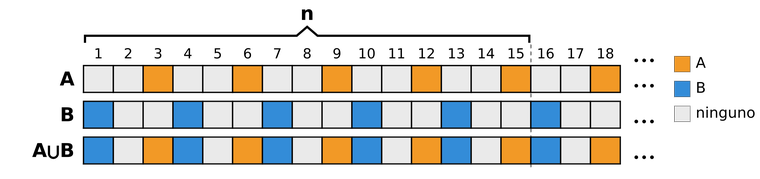
\includegraphics[width=0.75\linewidth]{imagenes/tema2/T2_P25_a.png}
\end{center}
\begin{center}
    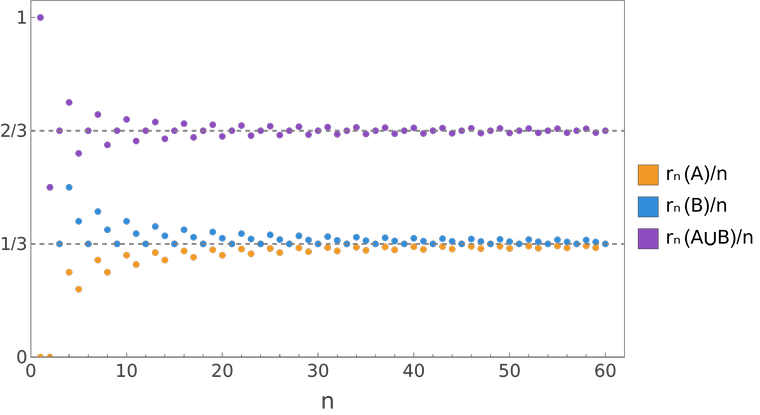
\includegraphics[width=0.75\linewidth]{imagenes/tema2/T2_P25_b.png}
\end{center}
\begin{center}
    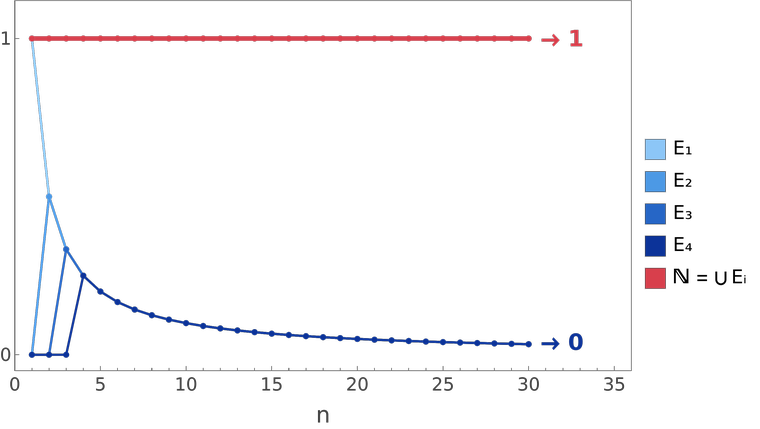
\includegraphics[width=0.75\linewidth]{imagenes/tema2/T2_P25_c.png}
\end{center}
\end{problema}

\newpage

% ------------------------------------------------------------------------------
% PROBLEMA 26
% ------------------------------------------------------------------------------
\begin{problema}[Continuidad de la medida de cardinal y cálculo de límites]
Tomemos $\Omega = \mathbb{N}$, $\mathcal{G} = \mathcal{P}(\mathbb{N})$ y la función de conjunto $\mu(A) = \text{cardinal}(A)$. Sea $\{A_n\}$ la sucesión de conjuntos con término general $A_n = \{x = 2m \mid m \le n\}$. ¿Podemos calcular $\mu\left(\lim_{n \to \infty} A_n\right)$ sin conocer el conjunto límite de la sucesión $\{A_n\}$?

\tcblower

Analizamos la naturaleza de la función de conjunto y de la sucesión:

\begin{enumerate}
    \item \textbf{Propiedades de la función de conjunto:} 
    La función $\mu(A) = \text{cardinal}(A)$ es una medida sobre el espacio medible $(\mathbb{N}, \mathcal{P}(\mathbb{N}))$, ya que es positiva y $\sigma$-aditiva. Por consiguiente, al ser una medida, es una función de conjunto continua (tanto ascendente como descendentemente).

    \item \textbf{Monotonía de la sucesión:} 
    El término general de la sucesión es $A_n = \{2, 4, 6, \dots, 2n\}$. Es evidente que cada conjunto está contenido en el siguiente:
    \[
        A_1 \subseteq A_2 \subseteq A_3 \subseteq \dots \subseteq A_n \subseteq \dots
    \]
    Por lo tanto, la sucesión $\{A_n\}$ es monótona creciente, lo que garantiza su convergencia.

    \item \textbf{Aplicación de la continuidad de la medida:} 
    Gracias a la propiedad de continuidad ascendente de las medidas, podemos conmutar la aplicación de la medida con el límite de la sucesión monótona:
    \[
        \mu\left( \lim_{n \to \infty} A_n \right) = \lim_{n \to \infty} \mu(A_n)
    \]
\end{enumerate}

Calculamos directamente el límite de las medidas de los términos individuales sin necesidad de determinar explícitamente el conjunto límite:
\[
    \mu(A_n) = \text{cardinal}(\{2, 4, \dots, 2n\}) = n
\]
Tomando el límite cuando $n \to \infty$:
\[
    \lim_{n \to \infty} \mu(A_n) = \lim_{n \to \infty} n = +\infty
\]

\textbf{Conclusión:} Sí es posible calcular $\mu\left(\lim_{n \to \infty} A_n\right)$ sin conocer explícitamente el conjunto límite (que en este caso correspondería al conjunto de los números pares $2\mathbb{N}$, de cardinal infinito), utilizando la propiedad de continuidad de la medida.
\begin{center}
    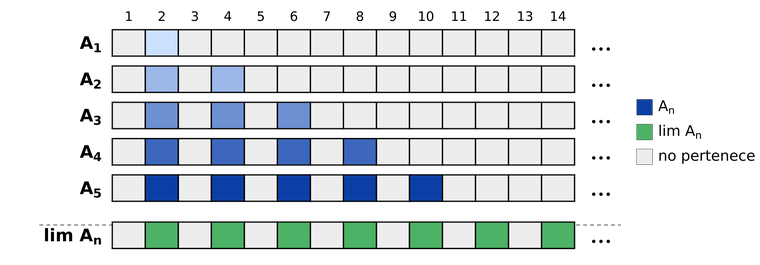
\includegraphics[width=0.75\linewidth]{imagenes/tema2/T2_P26_a.png}
\end{center}
\begin{center}
    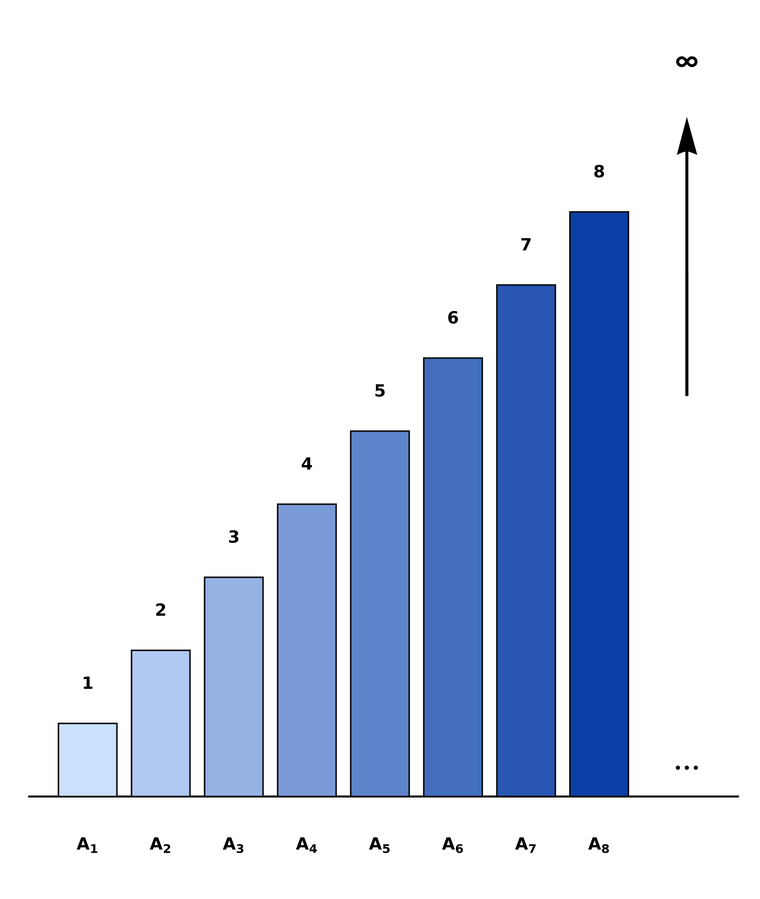
\includegraphics[width=0.75\linewidth]{imagenes/tema2/T2_P26_b.png}
\end{center}
\end{problema}

\newpage

% ------------------------------------------------------------------------------
% PROBLEMA 27
% ------------------------------------------------------------------------------
\begin{problema}[Falta de continuidad descendente cuando la medida es infinita]
Tomemos $\Omega = \mathbb{R}$, $\mathcal{G} = \mathcal{B}$ (la $\sigma$-álgebra de Borel) y la función de conjunto $\lambda(A) = \text{longitud del intervalo } A$ (medida de Lebesgue). Sea $\{A_n\}_{n \in \mathbb{N}}$ la sucesión de conjuntos definida por $A_n = (n, \infty)$. ¿Se verifica que $\lambda\left(\lim_{n \to \infty} A_n\right) = \lim_{n \to \infty} \lambda(A_n)$?

\tcblower

Calculamos independientemente ambos lados de la igualdad para comprobar si coinciden:

\begin{enumerate}
    \item \textbf{Cálculo del miembro izquierdo $\lambda\left(\lim_{n \to \infty} A_n\right)$:}
    
    La sucesión de intervalos $A_n = (n, \infty)$ es monótona decreciente, ya que:
    \[
        A_1 \supset A_2 \supset A_3 \supset \dots \supset A_n \supset A_{n+1} \supset \dots
    \]
    Por ser una sucesión decreciente, su límite de conjuntos viene dado por la intersección de todos sus términos:
    \[
        \lim_{n \to \infty} A_n = \bigcap_{n=1}^\infty (n, \infty) = \varnothing
    \]
    Puesto que la medida de Lebesgue del conjunto vacío es nula, obtenemos:
    \[
        \lambda\left( \lim_{n \to \infty} A_n \right) = \lambda(\varnothing) = 0
    \]

    \item \textbf{Cálculo del miembro derecho $\lim_{n \to \infty} \lambda(A_n)$:}
    
    Para todo $n \in \mathbb{N}$, el intervalo $A_n = (n, \infty)$ es un semieje no acotado, por lo que su medida de Lebesgue es infinita:
    \[
        \lambda(A_n) = \lambda((n, \infty)) = \infty, \quad \forall n \in \mathbb{N}
    \]
    Tomando el límite de la sucesión constante de medidas:
    \[
        \lim_{n \to \infty} \lambda(A_n) = \lim_{n \to \infty} \infty = \infty
    \]
\end{enumerate}

\paragraph{Conclusión:}
Puesto que $0 \neq \infty$, \textbf{no se verifica} la igualdad $\lambda\left(\lim_{n \to \infty} A_n\right) = \lim_{n \to \infty} \lambda(A_n)$.

\paragraph{Nota teórica:}
Aunque la medida de Lebesgue es $\sigma$-aditiva y por tanto continua, la propiedad de \textit{continuidad descendente} exige como hipótesis imprescindible que la medida de al menos un término de la sucesión sea finita ($\exists n_0 \text{ tal que } \lambda(A_{n_0}) < \infty$). Al ser $\lambda(A_n) = \infty$ para todo $n \in \mathbb{N}$, no se cumple esta condición necesaria y la medida no conmuta con el límite.
\end{problema}

\newpage

% ------------------------------------------------------------------------------
% PROBLEMA 28
% ------------------------------------------------------------------------------
\begin{problema}[Medida de Lebesgue de números sin el dígito 1 en su desarrollo decimal]
Determinar la medida de Lebesgue del conjunto $A \subset [0,1]$ formado por los números reales que en su escritura decimal no contienen ningún dígito igual a $1$.

\tcblower

Construimos el conjunto $A$ mediante una sucesión decreciente de conjuntos $\{A_n\}_{n \in \mathbb{N}_0}$:
\begin{align*}
    A_0 &= [0,1] \\
    A_1 &= \{ x \in [0,1] \mid \text{el primer dígito decimal de } x \text{ no es } 1 \} = [0, 1] \setminus [0.1, 0.2) \\
    A_2 &= \{ x \in [0,1] \mid \text{los dos primeros dígitos decimales de } x \text{ no son } 1 \} \\
    &\;\;\vdots \\
    A_n &= \{ x \in [0,1] \mid \text{ninguno de los primeros } n \text{ dígitos decimales de } x \text{ es } 1 \}
\end{align*}

El conjunto de interés se obtiene como la intersección numerable de esta familia:
\[
    A = \bigcap_{n=0}^\infty A_n = \lim_{n \to \infty} A_n
\]

% Espacio reservado para incorporar figura en los apuntes
\begin{center}
    \vspace{0.2cm}
    \framebox[\linewidth]{\vbox to 2.2cm{\vfill \centering \textit{[Espacio reservado para diagrama: Representación gráfica de los conjuntos $A_0, A_1, A_2$ en la recta real]} \vfill}}
    \vspace{0.2cm}
\end{center}

Calculamos la medida de Lebesgue $\lambda$ de los primeros términos:
\begin{itemize}
    \item $\lambda(A_0) = 1 = \left(\frac{9}{10}\right)^0$
    \item Para obtener $A_1$, retiramos de $A_0$ el intervalo $[0.1, 0.2)$ de longitud $1/10$. Por tanto:
    \[
        \lambda(A_1) = 1 - \frac{1}{10} = \frac{9}{10} = \left(\frac{9}{10}\right)^1
    \]
    \item Para obtener $A_2$, retiramos de $A_1$ los $9$ subintervalos de longitud $1/100$ cuyos segundos dígitos son $1$. La medida eliminada es $9 \cdot \frac{1}{100} = \frac{9}{100}$:
    \[
        \lambda(A_2) = \frac{9}{10} - \frac{9}{100} = \frac{81}{100} = \left(\frac{9}{10}\right)^2
    \]
    \item Por inducción, en la etapa $n$-ésima la medida de $A_n$ viene dada por:
    \[
        \lambda(A_n) = \left(\frac{9}{10}\right)^n
    \]
\end{itemize}

Puesto que $\{A_n\}$ es una sucesión decreciente de conjuntos ($A_n \downarrow$) y la medida del primer conjunto es finita ($\lambda(A_0) = 1 < \infty$), podemos aplicar el Teorema de continuidad de medidas (continuidad descendente):
\[
    \lambda(A) = \lambda\left( \lim_{n \to \infty} A_n \right) = \lim_{n \to \infty} \lambda(A_n) = \lim_{n \to \infty} \left(\frac{9}{10}\right)^n = 0
\]

Por tanto, la medida de Lebesgue del conjunto $A$ es nula ($\lambda(A) = 0$).
\end{problema}

% ------------------------------------------------------------------------------
% PROBLEMA 29
% ------------------------------------------------------------------------------
\begin{problema}[Verificación de continuidad para la medida cardinal en $\mathbb{N}$]
Sea el espacio de medida $(\mathbb{N}, \mathcal{P}(\mathbb{N}), \mu)$ con $\mu = \text{cardinal}$. Para las siguientes sucesiones de subconjuntos de $\mathbb{N}$:
\begin{enumerate}[label=\alph*)]
    \item $A_n = \{2n, 2n+2, 2n+4, \dots\}$
    \item $A_n = \{n, n+1, n+2, \dots, 2n\}$
\end{enumerate}
¿Se verifica que $\mu\left(\lim_{n \to \infty} A_n\right) = \lim_{n \to \infty} \mu(A_n)$?

\tcblower

\begin{enumerate}[label=\alph*)]
    \item \textbf{Análisis de la sucesión $A_n = \{2n, 2n+2, 2n+4, \dots\}$:}
    
    La sucesión $\{A_n\}$ es monótona decreciente ($A_1 \supset A_2 \supset A_3 \dots$), por lo que su límite de conjuntos existe y viene dado por la intersección de todos sus términos:
    \[
        \lim_{n \to \infty} A_n = \bigcap_{n=1}^\infty A_n = \varnothing \implies \mu\left( \lim_{n \to \infty} A_n \right) = \mu(\varnothing) = 0
    \]
    
    Analizamos si es posible conmutar la medida con el límite mediante el Teorema de continuidad:
    \begin{itemize}
        \item Para todo $n \in \mathbb{N}$, el cardinal de $A_n$ es infinito: $\mu(A_n) = \infty$.
        \item Al ser $\mu(A_n) = \infty$ para todo $n \in \mathbb{N}$, no se cumple la hipótesis de finitud de algún término ($\exists n_0 \text{ tal que } \mu(A_{n_0}) < \infty$). Por tanto, no es aplicable el Teorema de continuidad descendente.
    \end{itemize}
    
    Calculando directamente el límite numérico de las medidas:
    \[
        \lim_{n \to \infty} \mu(A_n) = \lim_{n \to \infty} \infty = \infty
    \]
    
    Dado que $0 \neq \infty$, \textbf{no se verifica} la igualdad $\mu\left(\lim_{n \to \infty} A_n\right) = \lim_{n \to \infty} \mu(A_n)$.

    \item \textbf{Análisis de la sucesión $A_n = \{n, n+1, n+2, \dots, 2n\}$:}
    
    La sucesión $\{A_n\}$ no es monótona ($A_1 = \{1,2\}$, $A_2 = \{2,3,4\}$, $A_3 = \{3,4,5,6\}$), por lo que debemos calcular sus límites superior e inferior de conjuntos:
    \begin{itemize}
        \item \textit{Límite superior:} La sucesión de uniones $\sigma_n = \bigcup_{j=n}^\infty A_j = \{n, n+1, n+2, \dots\}$ satisface:
        \[
            \varlimsup_{n \to \infty} A_n = \bigcap_{n=1}^\infty \sigma_n = \varnothing
        \]
        \item \textit{Límite inferior:} La sucesión de intersecciones $\delta_n = \bigcap_{j=n}^\infty A_j = \varnothing$ (pues ningún número pertenece a $A_j$ para todo $j \ge n$) satisface:
        \[
            \varliminf_{n \to \infty} A_n = \bigcup_{n=1}^\infty \delta_n = \varnothing
        \]
    \end{itemize}
    Al coincidir ambos límites, el límite de la sucesión de conjuntos existe y vale $\lim_{n \to \infty} A_n = \varnothing$, con lo cual:
    \[
        \mu\left( \lim_{n \to \infty} A_n \right) = \mu(\varnothing) = 0
    \]
    
    Comprobamos las hipótesis del Teorema de continuidad para medidas:
    Puesto que $\mu(\sigma_n) = \mu(\{n, n+1, \dots\}) = \infty$ para todo $n \in \mathbb{N}$, la hipótesis de medida finita sobre las uniones no se verifica y no se puede aplicar el teorema.
    
    Calculamos directamente el límite de las medidas de los términos:
    \[
        \mu(A_n) = \text{card}(\{n, n+1, \dots, 2n\}) = 2n - n + 1 = n + 1
    \]
    \[
        \lim_{n \to \infty} \mu(A_n) = \lim_{n \to \infty} (n + 1) = \infty
    \]
    
    Como $0 \neq \infty$, \textbf{tampoco se verifica} la igualdad en este apartado.
\end{enumerate}
\end{problema}
\newpage
% ------------------------------------------------------------------------------
% PROBLEMA 30
% ------------------------------------------------------------------------------
\begin{problema}[Comprobación del Teorema de continuidad para sucesiones de conjuntos unipuntuales]
Considerando la sucesión de subconjuntos de $\mathbb{R}$ dada por $A_n = \{n\}$, decidir qué desigualdades o igualdades del Teorema de continuidad para medidas se verifican para las siguientes medidas:
\begin{enumerate}[label=\alph*)]
    \item $\nu \equiv$ Probabilidad concentrada en $\mathbb{N}$.
    \item $\mu \equiv$ Cardinal (medida de contar).
\end{enumerate}

\tcblower

Calculamos en primer lugar el límite de la sucesión de conjuntos $A_n = \{n\}$:
\begin{itemize}
    \item $\sigma_n = \bigcup_{j=n}^\infty \{j\} = \{n, n+1, n+2, \dots\} \implies \varlimsup_{n \to \infty} A_n = \bigcap_{n=1}^\infty \sigma_n = \varnothing$
    \item $\delta_n = \bigcap_{j=n}^\infty \{j\} = \varnothing \implies \varliminf_{n \to \infty} A_n = \bigcup_{n=1}^\infty \delta_n = \varnothing$
\end{itemize}
Dado que $\varliminf_{n \to \infty} A_n = \varlimsup_{n \to \infty} A_n = \varnothing$, la sucesión es convergente y $\lim_{n \to \infty} A_n = \varnothing$.

\paragraph{Apartado a) Medida de probabilidad $\nu$ concentrada en $\mathbb{N}$:}
Al ser $\nu$ una medida de probabilidad, cumple $\nu(\mathbb{R}) = \nu(\mathbb{N}) = 1 < \infty$. Por tanto, el espacio de medida es finito y se satisfacen todas las hipótesis del Corolario de continuidad para probabilidades:

\begin{enumerate}[label=\arabic*.]
    \item Medida del conjunto límite: $\nu\left( \lim_{n \to \infty} A_n \right) = \nu(\varnothing) = 0$.
    \item Límite de las medidas: Dado que $\nu(\mathbb{N}) = \sum_{n=1}^\infty \nu(\{n\}) = 1 < \infty$, la serie converge y su término general tiende a cero, es decir, $\lim_{n \to \infty} \nu(A_n) = \lim_{n \to \infty} \nu(\{n\}) = 0$.
\end{enumerate}

Sustituyendo en la cadena de desigualdades del Teorema 6 / Corolario 1:
\[
    \nu\left( \varliminf_{n \to \infty} A_n \right) \le \varliminf_{n \to \infty} \nu(A_n) \le \varlimsup_{n \to \infty} \nu(A_n) \le \nu\left( \varlimsup_{n \to \infty} A_n \right)
\]
\[
    0 \le 0 \le 0 \le 0
\]
Se verifican todas las desigualdades, convirtiéndose en \textbf{igualdades estrictas} ($\nu(\lim A_n) = \lim \nu(A_n) = 0$).

\paragraph{Apartado b) Medida cardinal $\mu$:}
Evaluamos los términos de la cadena de desigualdades para la medida de contar $\mu$:
\begin{enumerate}[label=\arabic*.]
    \item Medida del límite inferior y superior de conjuntos:
    \[
        \mu\left( \varliminf_{n \to \infty} A_n \right) = \mu(\varnothing) = 0, \quad \mu\left( \varlimsup_{n \to \infty} A_n \right) = \mu(\varnothing) = 0
    \]
    \item Límites de las medidas numéricas:
    Como $\mu(A_n) = \text{card}(\{n\}) = 1$ para todo $n \in \mathbb{N}$, se tiene:
    \[
        \varliminf_{n \to \infty} \mu(A_n) = \lim_{n \to \infty} 1 = 1, \quad \varlimsup_{n \to \infty} \mu(A_n) = \lim_{n \to \infty} 1 = 1
    \]
\end{enumerate}

Analizamos la validez de la cadena de desigualdades:
\[
    \mu\left( \varliminf_{n \to \infty} A_n \right) \le \varliminf_{n \to \infty} \mu(A_n) \le \varlimsup_{n \to \infty} \mu(A_n) \le \mu\left( \varlimsup_{n \to \infty} A_n \right)
\]
Sustituyendo los valores calculados:
\[
    0 \le 1 \le 1 \le 0
\]
Concluimos que:
\begin{itemize}
    \item Las dos primeras desigualdades de la parte general del Teorema 6a ($0 \le 1 \le 1$) \textbf{sí se verifican}.
    \item La última desigualdad ($1 \le 0$) \textbf{falla} y no se cumple. Esto es consistente con la teoría, pues $\mu(\sigma_n) = \mu(\{n, n+1, \dots\}) = \infty$, incumpliéndose la hipótesis del Teorema 6b de finitud de la medida sobre la cola de uniones.
\end{itemize}
\end{problema}
\newpage
% ------------------------------------------------------------------------------
% PROBLEMA 31
% ------------------------------------------------------------------------------
\begin{problema}[$\sigma$-finitud en sub-$\sigma$-álgebras]
Sea $(\Omega, \mathcal{G}, \mu)$ un espacio de medida $\sigma$-finito y sea $\mathcal{F}$ una $\sigma$-álgebra contenida en $\mathcal{G}$ ($\mathcal{F} \subseteq \mathcal{G}$). ¿Es $(\Omega, \mathcal{F}, \mu)$ un espacio de medida $\sigma$-finito? En caso de respuesta negativa, encontrar un contraejemplo.

\tcblower

\paragraph{Respuesta:}
No necesariamente. La propiedad de $\sigma$-finitud exige no solo que la medida $\mu$ permita recubrir el espacio $\Omega$ mediante conjuntos de medida finita, sino que dichos conjuntos pertenezcan explícitamente a la $\sigma$-álgebra considerada. Si la sub-$\sigma$-álgebra $\mathcal{F}$ es demasiado gruesa (poco fina), puede no contener suficientes subconjuntos de medida finita para cubrir todo el espacio $\Omega$.

\paragraph{Contraejemplo:}
Consideremos el espacio muestral numerable $\Omega = \mathbb{N}$ equipado con la $\sigma$-álgebra de las partes $\mathcal{G} = \mathcal{P}(\mathbb{N})$ y la medida cardinal o de contar $\mu = \text{cardinal}$.

\begin{enumerate}
    \item \textbf{$(\Omega, \mathcal{G}, \mu)$ es $\sigma$-finito:}
    Podemos expresar $\mathbb{N}$ como la unión numerable de subconjuntos unipuntuales $A_n = \{n\} \in \mathcal{P}(\mathbb{N})$:
    \[
        \mathbb{N} = \bigcup_{n=1}^\infty \{n\}
    \]
    donde cada término satisface $\mu(\{n\}) = 1 < \infty$. Por consiguiente, $(\mathbb{N}, \mathcal{P}(\mathbb{N}), \mu)$ es un espacio de medida $\sigma$-finito.

    \item \textbf{Elección de la sub-$\sigma$-álgebra $\mathcal{F}$:}
    Tomamos como sub-$\sigma$-álgebra la $\sigma$-álgebra trivial sobre $\mathbb{N}$:
    \[
        \mathcal{F} = \{\varnothing, \mathbb{N}\} \subseteq \mathcal{P}(\mathbb{N})
    \]
    
    \item \textbf{$(\Omega, \mathcal{F}, \mu)$ no es $\sigma$-finito:}
    Evaluamos la medida $\mu$ sobre los únicos dos elementos que pertenecen a $\mathcal{F}$:
    \[
        \mu(\varnothing) = 0 < \infty, \quad \mu(\mathbb{N}) = \text{cardinal}(\mathbb{N}) = \infty
    \]
    Para que $(\mathbb{N}, \mathcal{F}, \mu)$ fuese un espacio $\sigma$-finito, tendría que existir una sucesión de conjuntos $\{E_n\}_{n \in \mathbb{N}} \subseteq \mathcal{F}$ con $\mu(E_n) < \infty$ para todo $n$ tal que $\bigcup_{n=1}^\infty E_n = \mathbb{N}$.
    
    Sin embargo, el único conjunto de la sub-$\sigma$-álgebra $\mathcal{F}$ que posee medida finita es el conjunto vacío ($E_n = \varnothing$). La unión numerable de conjuntos vacíos satisface:
    \[
        \bigcup_{n=1}^\infty \varnothing = \varnothing \neq \mathbb{N}
    \]
    
    Por lo tanto, es imposible recubrir $\mathbb{N}$ con elementos de $\mathcal{F}$ que tengan medida finita.
\end{enumerate}

% Espacio reservado para incorporar diagrama explicativo en los apuntes
\begin{center}
    \vspace{0.2cm}
    \framebox[\linewidth]{\vbox to 2.2cm{\vfill \centering \textit{[Espacio reservado para diagrama: Comparación de la partición fina en $\mathcal{P}(\mathbb{N})$ frente al bloque único de la sub-$\sigma$-álgebra trivial $\mathcal{F}=\{\varnothing, \mathbb{N}\}$]} \vfill}}
    \vspace{0.2cm}
\end{center}

\paragraph{Conclusión:}
El par $(\Omega, \mathcal{F}, \mu)$ no es un espacio de medida $\sigma$-finito. La $\sigma$-finitud depende críticamente de la $\sigma$-álgebra sobre la que se evalúa la medida y no se conserva necesariamente al restringirse a una sub-$\sigma$-álgebra.
\end{problema}
\newpage
% ------------------------------------------------------------------------------
% PROBLEMA 32
% ------------------------------------------------------------------------------
\begin{problema}[Medida concentrada en $\mathbb{N}$ y singularidad mutua con Lebesgue]
Sea $\Omega = \mathbb{R}$, $\mathcal{B}$ la $\sigma$-álgebra de Borel sobre $\mathbb{R}$ y $\lambda$ la medida de Lebesgue. Demostrar que la función de conjunto
\[
    \nu(A) = \#(A \cap \mathbb{N})
\]
(que cuenta el número de enteros positivos pertenecientes a $A$) es una medida sobre $(\mathbb{R}, \mathcal{B})$ y que las medidas $\lambda$ y $\nu$ son mutuamente singulares ($\lambda \perp \nu$).

\tcblower

\paragraph{1. Comprobación de que $\nu$ es una medida sobre $(\mathbb{R}, \mathcal{B})$:}
Verificamos los axiomas de medida sobre el espacio medible $(\mathbb{R}, \mathcal{B})$:
\begin{enumerate}[label=\alph*)]
    \item \textit{No negatividad:} Para todo conjunto $A \in \mathcal{B}$, la intersección $A \cap \mathbb{N}$ es un subconjunto de naturales, por lo que su cardinal es no negativo:
    \[
        \nu(A) = \#(A \cap \mathbb{N}) \ge 0, \quad \forall A \in \mathcal{B}
    \]
    \item \textit{Medida del conjunto vacío:} Para $A = \varnothing$, se cumple $\varnothing \cap \mathbb{N} = \varnothing$, de donde:
    \[
        \nu(\varnothing) = \#(\varnothing) = 0
    \]
    \item \textit{$\sigma$-aditividad:} Dada una sucesión $(A_n)_{n \in \mathbb{N}} \subseteq \mathcal{B}$ de conjuntos borelianos disjuntos dos a dos ($A_i \cap A_j = \varnothing$ para todo $i \neq j$), la distribución del producto cartesiano/intersección satisface que los conjuntos $(A_n \cap \mathbb{N})_{n \in \mathbb{N}}$ son también disjuntos dos a dos. Por la aditividad del cardinal sobre conjuntos disjuntos:
    \[
        \nu\left( \bigcup_{n=1}^\infty A_n \right) = \#\left( \left(\bigcup_{n=1}^\infty A_n\right) \cap \mathbb{N} \right) = \#\left( \bigcup_{n=1}^\infty (A_n \cap \mathbb{N}) \right) = \sum_{n=1}^\infty \#(A_n \cap \mathbb{N}) = \sum_{n=1}^\infty \nu(A_n)
    \]
\end{enumerate}
Por tanto, $\nu$ es una medida sobre $(\mathbb{R}, \mathcal{B})$ (medida de contar concentrada en $\mathbb{N}$).

\paragraph{2. Demostración de que $\lambda$ y $\nu$ son mutuamente singulares ($\lambda \perp \nu$):}
Por definición, $\lambda \perp \nu$ si existe un conjunto medible $A \in \mathcal{B}$ tal que $\nu(A) = 0$ y $\lambda(A^c) = 0$.

Consideremos el conjunto de los números irracionales y no enteros positivos, o equivalentemente, el complementario de los números naturales en la recta real:
\[
    A = \mathbb{N}^c = \mathbb{R} \setminus \mathbb{N} \in \mathcal{B}
\]

Evaluamos ambas medidas sobre el conjunto $A$ y su complementario $A^c = \mathbb{N}$:
\begin{itemize}
    \item \textit{Medida $\nu$ sobre $A$:} 
    \[
        \nu(A) = \nu(\mathbb{R} \setminus \mathbb{N}) = \#\left((\mathbb{R} \setminus \mathbb{N}) \cap \mathbb{N}\right) = \#(\varnothing) = 0
    \]
    \item \textit{Medida de Lebesgue $\lambda$ sobre $A^c$:}
    El complementario es $A^c = \mathbb{N} = \bigcup_{n=1}^\infty \{n\}$, un conjunto numerable de puntos aislados. Dado que la medida de Lebesgue de cualquier singleton es nula ($\lambda(\{n\}) = 0$), por $\sigma$-aditividad de $\lambda$:
    \[
        \lambda(A^c) = \lambda(\mathbb{N}) = \sum_{n=1}^\infty \lambda(\{n\}) = \sum_{n=1}^\infty 0 = 0
    \]
\end{itemize}

% Espacio reservado para incorporar diagrama explicativo en los apuntes
\begin{center}
    \vspace{0.2cm}
    \framebox[\linewidth]{\vbox to 2.2cm{\vfill \centering \textit{[Espacio reservado para diagrama: Soporte discreto $\mathbb{N}$ de la medida $\nu$ frente al soporte continuo de la medida de Lebesgue $\lambda$]} \vfill}}
    \vspace{0.2cm}
\end{center}

Al haber encontrado un suceso $A = \mathbb{N}^c \in \mathcal{B}$ tal que $\nu(A) = 0$ y $\lambda(A^c) = 0$, queda demostrado que las medidas $\lambda$ y $\nu$ son mutuamente singulares ($\lambda \perp \nu$).
\end{problema}
\newpage
% ------------------------------------------------------------------------------
% PROBLEMA 33
% ------------------------------------------------------------------------------
\begin{problema}[Relación de continuidad absoluta entre la medida de Lebesgue y la medida cardinal]
Sea $\Omega = \mathbb{R}$, $\mathcal{B}$ la $\sigma$-álgebra de Borel, $\lambda$ la medida de Lebesgue y $\nu$ la medida cardinal (de contar) sobre $\mathbb{R}$. Decidir si se verifica $\lambda \ll \nu$ o $\nu \ll \lambda$.

\tcblower

Analizamos por separado ambas direcciones de la relación de continuidad absoluta:

\paragraph{1. Estudio de $\nu \ll \lambda$ (Continuidad absoluta de la medida cardinal respecto a Lebesgue):}
Para que la medida cardinal $\nu$ fuese absolutamente continua respecto a la medida de Lebesgue $\lambda$, se tendría que verificar la implicación:
\[
    \forall A \in \mathcal{B}, \quad \lambda(A) = 0 \implies \nu(A) = 0
\]
Consideremos el conjunto unipuntual formado por el número cero, $A = \{0\} \in \mathcal{B}$:
\begin{itemize}
    \item La medida de Lebesgue de un punto es nula: $\lambda(\{0\}) = 0$.
    \item La medida cardinal de un punto es su número de elementos: $\nu(\{0\}) = \text{card}(\{0\}) = 1$.
\end{itemize}
Dado que $\lambda(\{0\}) = 0$ pero $\nu(\{0\}) = 1 \neq 0$, la implicación no se cumple.
Por lo tanto, \textbf{$\nu$ no es absolutamente continua respecto a $\lambda$} ($\nu \not\ll \lambda$).

% Espacio reservado para incorporar diagrama explicativo en los apuntes
\begin{center}
    \vspace{0.2cm}
    \framebox[\linewidth]{\vbox to 2.2cm{\vfill \centering \textit{[Espacio reservado para diagrama: Contrapunto entre medida nula de Lebesgue en un singleton y su medida cardinal no nula]} \vfill}}
    \vspace{0.2cm}
\end{center}

\paragraph{2. Estudio de $\lambda \ll \nu$ (Continuidad absoluta de Lebesgue respecto a la medida cardinal):}
Para comprobar si la medida de Lebesgue $\lambda$ es absolutamente continua respecto a la medida cardinal $\nu$, analizamos la condición:
\[
    \forall A \in \mathcal{B}, \quad \nu(A) = 0 \implies \lambda(A) = 0
\]
Por definición, la medida cardinal de un conjunto $A \subseteq \mathbb{R}$ es cero si y solo si $A$ no contiene ningún elemento, es decir, únicamente cuando $A$ es el conjunto vacío:
\[
    \nu(A) = 0 \iff A = \varnothing
\]
Evaluando la medida de Lebesgue sobre el conjunto vacío:
\[
    \lambda(\varnothing) = 0
\]
Dado que la única forma de que $\nu(A)$ se anule es que $A = \varnothing$, y sobre dicho conjunto la medida de Lebesgue $\lambda$ se anula trivialmente, la implicación $\nu(A) = 0 \implies \lambda(A) = 0$ se satisface universalmente para todo $A \in \mathcal{B}$.

Por lo tanto, \textbf{$\lambda$ es absolutamente continua respecto a $\nu$} ($\lambda \ll \nu$).
\end{problema}
\newpage
% ------------------------------------------------------------------------------
% PROBLEMA 34
% ------------------------------------------------------------------------------
\begin{problema}[Medidas inducidas por restricciones de Lebesgue a semiejes y comparación]
Sea $\Omega = \mathbb{R}$, $\mathcal{B}$ la $\sigma$-álgebra de Borel y $\lambda$ la medida de Lebesgue. Determinar si las funciones de conjunto definidas para cada $B \in \mathcal{B}$ por:
\[
    \mu(B) = \lambda(B \cap \mathbb{R}^-) \quad \text{y} \quad \nu(B) = \lambda(B \cap \mathbb{R}^+)
\]
donde $\mathbb{R}^- = (-\infty, 0)$ y $\mathbb{R}^+ = [0, \infty)$, son medidas sobre $(\mathbb{R}, \mathcal{B})$.

Decidir si son mutuamente singulares o absolutamente continuas la una respecto de la otra, y analizar su relación de continuidad absoluta respecto de la medida de Lebesgue $\lambda$.

\tcblower

\paragraph{1. Comprobación de la estructura de medida:}
Comprobamos los axiomas de medida sobre $(\mathbb{R}, \mathcal{B})$ para la función de conjunto $\mu$ (el caso de $\nu$ es completamente análogo):
\begin{enumerate}[label=\alph*)]
    \item \textit{No negatividad:} Como la medida de Lebesgue es positiva, para todo $B \in \mathcal{B}$ se cumple:
    \[
        \mu(B) = \lambda(B \cap \mathbb{R}^-) \ge 0
    \]
    \item \textit{Medida del conjunto vacío:} 
    \[
        \mu(\varnothing) = \lambda(\varnothing \cap \mathbb{R}^-) = \lambda(\varnothing) = 0
    \]
    \item \textit{$\sigma$-aditividad:} Dada una sucesión $(B_n)_{n \in \mathbb{N}} \subseteq \mathcal{B}$ de conjuntos disjuntos dos a dos ($B_i \cap B_j = \varnothing$ para $i \neq j$), la familia $(B_n \cap \mathbb{R}^-)_{n \in \mathbb{N}}$ es también disjunta dos a dos. Por la $\sigma$-aditividad de la medida de Lebesgue:
    \[
        \mu\left( \bigcup_{n=1}^\infty B_n \right) = \lambda\left( \left(\bigcup_{n=1}^\infty B_n\right) \cap \mathbb{R}^- \right) = \lambda\left( \bigcup_{n=1}^\infty (B_n \cap \mathbb{R}^-) \right) = \sum_{n=1}^\infty \lambda(B_n \cap \mathbb{R}^-) = \sum_{n=1}^\infty \mu(B_n)
    \]
\end{enumerate}
Por consiguiente, $\mu$ y $\nu$ son medidas bien definidas sobre $(\mathbb{R}, \mathcal{B})$.

\paragraph{2. Comparación entre $\mu$ y $\nu$:}
\begin{itemize}
    \item \textit{Singularidad mutua ($\mu \perp \nu$):}
    Consideremos el conjunto boreliano $A = \mathbb{R}^- = (-\infty, 0) \in \mathcal{B}$. Evaluamos ambas medidas sobre $A$ y su complementario $A^c = \mathbb{R}^+ = [0, \infty)$:
    \[
        \nu(A) = \lambda((-\infty, 0) \cap [0, \infty)) = \lambda(\varnothing) = 0
    \]
    \[
        \mu(A^c) = \lambda([0, \infty) \cap (-\infty, 0)) = \lambda(\varnothing) = 0
    \]
    Al existir un conjunto $A \in \mathcal{B}$ tal que $\nu(A) = 0$ y $\mu(A^c) = 0$, queda demostrado que las medidas $\mu$ y $\nu$ son mutuamente singulares ($\mu \perp \nu$).

    \item \textit{Continuidad absoluta recíproca:}
    Al ser medidas mutuamente singulares no nulas, no son absolutamente continuas entre sí. En efecto:
    \begin{itemize}
        \item Tomando $B_1 = (-1, 0)$, se tiene $\mu(B_1) = 1 > 0$ pero $\nu(B_1) = 0$, luego $\mu \not\ll \nu$.
        \item Tomando $B_2 = (0, 1)$, se tiene $\nu(B_2) = 1 > 0$ pero $\mu(B_2) = 0$, luego $\nu \not\ll \mu$.
    \end{itemize}
\end{itemize}

% Espacio reservado para incorporar diagrama explicativo en los apuntes
\begin{center}
    \vspace{0.2cm}
    \framebox[\linewidth]{\vbox to 2.2cm{\vfill \centering \textit{[Espacio reservado para diagrama: Soporte disjunto de las medidas $\mu$ sobre $(-\infty,0)$ y $\nu$ sobre $[0,\infty)$]} \vfill}}
    \vspace{0.2cm}
\end{center}

\paragraph{3. Comparación respecto de la medida de Lebesgue $\lambda$:}
\begin{itemize}
    \item \textit{Continuidad absoluta de $\mu$ y $\nu$ respecto de $\lambda$ ($\mu \ll \lambda$ y $\nu \ll \lambda$):}
    Sea $B \in \mathcal{B}$ tal que $\lambda(B) = 0$. Por la propiedad de monotonía de la medida de Lebesgue:
    \[
        B \cap \mathbb{R}^- \subseteq B \implies \mu(B) = \lambda(B \cap \mathbb{R}^-) \le \lambda(B) = 0 \implies \mu(B) = 0
    \]
    Analogamente, $\nu(B) = \lambda(B \cap \mathbb{R}^+) \le \lambda(B) = 0 \implies \nu(B) = 0$.
    Por tanto, se verifica que $\mu \ll \lambda$ y $\nu \ll \lambda$.

    \item \textit{Relación recíproca ($\lambda \not\ll \mu$ y $\lambda \not\ll \nu$):}
    La medida de Lebesgue no es absolutamente continua respecto de $\mu$ ni de $\nu$:
    \begin{itemize}
        \item Para $B_2 = (0, 1)$, $\mu(B_2) = 0$ pero $\lambda(B_2) = 1 \neq 0 \implies \lambda \not\ll \mu$.
        \item Para $B_1 = (-1, 0)$, $\nu(B_1) = 0$ pero $\lambda(B_1) = 1 \neq 0 \implies \lambda \not\ll \nu$.
    \end{itemize}
\end{itemize}

\paragraph{Nota adicional:}
Observamos que $\lambda = \mu + \nu$, lo que representa la descomposición de la medida de Lebesgue en sus componentes concentradas sobre los semiejes real negativo y real positivo.
\end{problema}

\newpage
\newpage %===

% ------------------------------------------------------------------------------
% PROBLEMA 35
% ------------------------------------------------------------------------------
\begin{problema}[Singularidad mutua entre una medida discreta de soporte finito y la medida de Lebesgue]
Sea $\Omega = \mathbb{R}$, $\mathcal{B}$ la $\sigma$-álgebra de Borel y $\lambda$ la medida de Lebesgue. Demostrar que toda medida discreta $\mu$ con soporte en $\{x_1, \dots, x_n\}$ definida sobre $(\mathbb{R}, \mathcal{B})$ (es decir, tal que $\mu(\{x\}) = 0$ para todo $x \notin \{x_1, \dots, x_n\}$) es mutuamente singular a $\lambda$.

\tcblower

Para demostrar que la medida discreta $\mu$ y la medida de Lebesgue $\lambda$ son mutuamente singulares ($\mu \perp \lambda$), debemos encontrar un conjunto medible $A \in \mathcal{B}$ tal que:
\[
    \mu(A) = 0 \quad \text{y} \quad \lambda(A^c) = 0
\]

Consideremos el soporte de la medida $\mu$, dado por el conjunto finito $S = \{x_1, \dots, x_n\} \in \mathcal{B}$, y definamos $A$ como el complementario de dicho soporte:
\[
    A = S^c = \mathbb{R} \setminus \{x_1, \dots, x_n\} \in \mathcal{B}
\]

Evaluamos el valor de ambas medidas sobre el conjunto $A$ y sobre su complementario $A^c = S$:

\paragraph{1. Medida $\mu$ sobre $A$:}
Por hipótesis, la medida $\mu$ está totalmente concentrada en los puntos $\{x_1, \dots, x_n\}$, por lo que la medida del complementario de su soporte es nula:
\[
    \mu(A) = \mu(\mathbb{R} \setminus \{x_1, \dots, x_n\}) = 0
\]

\paragraph{2. Medida de Lebesgue $\lambda$ sobre $A^c$:}
El complementario es $A^c = S = \{x_1, \dots, x_n\}$, que se descompone como la unión finita disjunta de puntos aislados:
\[
    A^c = \bigsqcup_{i=1}^n \{x_i\}
\]
Dado que la medida de Lebesgue de cualquier conjunto unipuntual es cero ($\lambda(\{x_i\}) = 0$ para todo $i$), aplicando la aditividad finita de $\lambda$:
\[
    \lambda(A^c) = \lambda\left( \bigsqcup_{i=1}^n \{x_i\} \right) = \sum_{i=1}^n \lambda(\{x_i\}) = \sum_{i=1}^n 0 = 0
\]

% Espacio reservado para incorporar diagrama explicativo en los apuntes
\begin{center}
    \vspace{0.2cm}
    \framebox[\linewidth]{\vbox to 2.2cm{\vfill \centering \textit{[Espacio reservado para diagrama: Soporte puntual $S=\{x_1,\dots,x_n\}$ de la medida discreta $\mu$ frente a la medida de Lebesgue $\lambda$]} \vfill}}
    \vspace{0.2cm}
\end{center}

Al haber encontrado el conjunto $A = S^c \in \mathcal{B}$ tal que $\mu(A) = 0$ y $\lambda(A^c) = 0$, queda demostrado que la medida discreta $\mu$ y la medida de Lebesgue $\lambda$ son mutuamente singulares ($\mu \perp \lambda$).

\paragraph{Análisis de la continuidad absoluta:}
De forma adicional, se observa que $\mu$ no es absolutamente continua respecto de $\lambda$ ($\mu \not\ll \lambda$). Tomando el conjunto del soporte $S = \{x_1, \dots, x_n\}$, tenemos que $\lambda(S) = 0$, pero $\mu(S) = \mu(\mathbb{R}) > 0$ (asumiendo que $\mu$ no es la medida nula). Por tanto, no se cumple la implicación de continuidad absoluta.
\end{problema}

\newpage
\newpage %===

% ------------------------------------------------------------------------------
% PROBLEMA 36
% ------------------------------------------------------------------------------
\begin{problema}[Medida definida mediante integral de densidad y continuidad absoluta]
Sea $\Omega = \mathbb{R}$, $\mathcal{B}$ la $\sigma$-álgebra de Borel y $\lambda$ la medida de Lebesgue. Demostrar que una función de conjunto definida sobre $(\mathbb{R}, \mathcal{B})$ como
\[
    \mu(A) = \int_A f(x) \, dx
\]
siendo $f(x) \ge 0$ para todo $x \in \mathbb{R}$, es una medida sobre $(\mathbb{R}, \mathcal{B})$. ¿Se verifica que $\lambda \ll \mu$ o $\mu \ll \lambda$?

\tcblower

\paragraph{1. Demostración de que $\mu$ es una medida sobre $(\mathbb{R}, \mathcal{B})$:}
Verificamos las tres propiedades fundamentales de las medidas sobre el espacio medible $(\mathbb{R}, \mathcal{B})$:
\begin{enumerate}[label=\alph*)]
    \item \textit{No negatividad:} Como $f(x) \ge 0$ para todo $x \in \mathbb{R}$, la integral de Lebesgue de una función no negativa sobre cualquier conjunto medible $A \in \mathcal{B}$ es no negativa:
    \[
        \mu(A) = \int_A f(x) \, dx \ge 0, \quad \forall A \in \mathcal{B}
    \]
    \item \textit{Medida del conjunto vacío:} Para $A = \varnothing$, la integral sobre un dominio de medida nula es cero:
    \[
        \mu(\varnothing) = \int_\varnothing f(x) \, dx = 0
    \]
    \item \textit{$\sigma$-aditividad:} Dada una sucesión $(A_n)_{n \in \mathbb{N}} \subseteq \mathcal{B}$ de conjuntos borelianos disjuntos dos a dos ($A_i \cap A_j = \varnothing$ para todo $i \neq j$), por la propiedad de la integral de Lebesgue (o el Teorema de convergencia monótona aplicado a la serie de funciones indicatrices):
    \[
        \mu\left( \bigcup_{n=1}^\infty A_n \right) = \int_{\bigcup_{n=1}^\infty A_n} f(x) \, dx = \int_{\mathbb{R}} \sum_{n=1}^\infty f(x) \chi_{A_n}(x) \, dx = \sum_{n=1}^\infty \int_{A_n} f(x) \, dx = \sum_{n=1}^\infty \mu(A_n)
    \]
\end{enumerate}
Por tanto, $\mu$ es una medida bien definida sobre $(\mathbb{R}, \mathcal{B})$.

\paragraph{2. Análisis de la relación $\mu \ll \lambda$:}
Estudiamos la condición $\forall A \in \mathcal{B}, \, \lambda(A) = 0 \implies \mu(A) = 0$.
Sea $A \in \mathcal{B}$ tal que $\lambda(A) = 0$. Por las propiedades generales de la integral de Lebesgue, la integral de cualquier función medible sobre un conjunto de medida de Lebesgue nula es siempre cero:
\[
    \mu(A) = \int_A f(x) \, d\lambda = 0
\]
Por consiguiente, \textbf{siempre se verifica que} $\mu \ll \lambda$ (la medida $\mu$ es absolutamente continua respecto de la medida de Lebesgue $\lambda$). En este contexto, la función $f$ actúa como la derivada de Radon-Nikodym de $\mu$ respecto de $\lambda$ ($f = \frac{d\mu}{d\lambda}$).

% Espacio reservado para incorporar diagrama explicativo en los apuntes
\begin{center}
    \vspace{0.2cm}
    \framebox[\linewidth]{\vbox to 2.2cm{\vfill \centering \textit{[Espacio reservado para diagrama: Integración de la función de densidad $f(x) \ge 0$ sobre conjuntos $A$ con medida de Lebesgue nula o positiva]} \vfill}}
    \vspace{0.2cm}
\end{center}

\paragraph{3. Análisis de la relación $\lambda \ll \mu$:}
Estudiamos si es cierto que $\forall A \in \mathcal{B}, \, \mu(A) = 0 \implies \lambda(A) = 0$.
Esta propiedad \textbf{no se verifica en general}, salvo que la densidad $f(x)$ sea estrictamente positiva casi por todas partes ($f(x) > 0$ c.s. $\lambda$).

\textit{Contraejemplo:} Consideremos la función $f(x) = 0$ para todo $x \in \mathbb{R}$ (o bien $f(x) = \chi_{[0, \infty)}(x)$).
Para $A = (-2, -1) \in \mathcal{B}$:
\begin{itemize}
    \item La medida $\mu$ del conjunto $A$ vale:
    \[
        \mu(A) = \int_{-2}^{-1} 0 \, dx = 0
    \]
    \item La medida de Lebesgue del conjunto $A$ vale:
    \[
        \lambda(A) = \lambda((-2, -1)) = 1 \neq 0
    \]
\end{itemize}
Dado que $\mu(A) = 0$ pero $\lambda(A) = 1 \neq 0$, la implicación de continuidad absoluta no se satisface.

Por tanto, en general \textbf{$\lambda$ no es absolutamente continua respecto de $\mu$} ($\lambda \not\ll \mu$).
\end{problema}

\newpage
\newpage %===

% ------------------------------------------------------------------------------
% PROBLEMA 37
% ------------------------------------------------------------------------------
\begin{problema}[Nulidad de una medida absolutamente continua y mutuamente singular]
Sean $\lambda, \mu : (\Omega, \mathcal{G}) \to \mathbb{R}$ dos medidas sobre el espacio medible $(\Omega, \mathcal{G})$. Demostrar que si $\lambda \ll \mu$ y $\lambda \perp \mu$, entonces $\lambda \equiv 0$ (la medida $\lambda$ es idénticamente nula).

\tcblower

\paragraph{1. Hipótesis de singularidad mutua ($\lambda \perp \mu$):}
Por definición de medidas mutuamente singulares, existe un conjunto medible $B_0 \in \mathcal{G}$ tal que:
\[
    \lambda(B_0) = 0 \quad \text{y} \quad \mu(B_0^c) = 0
\]

\paragraph{2. Aplicación de la continuidad absoluta ($\lambda \ll \mu$):}
La relación de continuidad absoluta establece que todo conjunto de medida nula según $\mu$ tiene también medida nula según $\lambda$:
\[
    \forall B \in \mathcal{G}, \quad \mu(B) = 0 \implies \lambda(B) = 0
\]
Aplicando esta implicación al conjunto $B_0^c \in \mathcal{G}$, dado que $\mu(B_0^c) = 0$, deducimos directamente que:
\[
    \lambda(B_0^c) = 0
\]

\paragraph{3. Medida del espacio total $\Omega$:}
Descomponemos el espacio muestral $\Omega$ en la unión disjunta de $B_0$ y su complementario $B_0^c$:
\[
    \Omega = B_0 \sqcup B_0^c
\]
Por la aditividad de la medida $\lambda$:
\[
    \lambda(\Omega) = \lambda(B_0 \sqcup B_0^c) = \lambda(B_0) + \lambda(B_0^c) = 0 + 0 = 0
\]

% Espacio reservado para incorporar diagrama explicativo en los apuntes
\begin{center}
    \vspace{0.2cm}
    \framebox[\linewidth]{\vbox to 2.2cm{\vfill \centering \textit{[Espacio reservado para diagrama: Intersección trivial de las condiciones de continuidad absoluta y singularidad mutua entre medidas]} \vfill}}
    \vspace{0.2cm}
\end{center}

\paragraph{4. Conclusión para un conjunto medible arbitrario:}
Para todo suceso $A \in \mathcal{G}$, la inclusión $A \subseteq \Omega$ implica, por la propiedad de monotonía de las medidas:
\[
    0 \le \lambda(A) \le \lambda(\Omega) = 0 \implies \lambda(A) = 0
\]
Dado que $\lambda(A) = 0$ para todo $A \in \mathcal{G}$, se concluye que la medida $\lambda$ es idénticamente nula ($\lambda \equiv 0$).
\end{problema}

\newpage
\newpage %===

% ------------------------------------------------------------------------------
% PROBLEMA 38
% ------------------------------------------------------------------------------
\begin{problema}[Propiedades algebraicas de la continuidad absoluta y la singularidad mutua]
Sean $\lambda_1, \lambda_2$ y $\mu$ tres medidas completas sobre el espacio medible $(\Omega, \mathcal{G})$. Demostrar las siguientes propiedades:
\begin{enumerate}[label=\alph*)]
    \item Si $\lambda_1 \ll \mu$ y $\lambda_2 \perp \mu$, entonces $\lambda_1 \perp \lambda_2$.
    \item Si $\lambda_1 \ll \mu$ y $\lambda_2 \ll \mu$, entonces $\lambda_1 + \lambda_2 \ll \mu$.
    \item Si $\lambda_1 \perp \mu$ y $\lambda_2 \perp \mu$, entonces $\lambda_1 + \lambda_2 \perp \mu$.
    \item Si $\lambda = \lambda_1 + \lambda_2$, entonces $\lambda_1 \ll \lambda$ y $\lambda_2 \ll \lambda$; y si además $\lambda_1 \ll \lambda_2$, entonces $\lambda \ll \lambda_2$.
\end{enumerate}

\tcblower

\paragraph{a) Demostración de $\lambda_1 \ll \mu \land \lambda_2 \perp \mu \implies \lambda_1 \perp \lambda_2$:}
Puesto que $\lambda_2 \perp \mu$, por definición de medidas mutuamente singulares, existe un conjunto medible $B_0 \in \mathcal{G}$ tal que:
\[
    \mu(B_0) = 0 \quad \text{y} \quad \lambda_2(B_0^c) = 0
\]
Por otro lado, como $\lambda_1 \ll \mu$, la medida $\lambda_1$ se anula sobre todo conjunto de medida nula según $\mu$. Aplicando esta propiedad al conjunto $B_0$:
\[
    \mu(B_0) = 0 \implies \lambda_1(B_0) = 0
\]
Por lo tanto, hemos encontrado un suceso $B_0 \in \mathcal{G}$ tal que $\lambda_1(B_0) = 0$ y $\lambda_2(B_0^c) = 0$, lo que demuestra que $\lambda_1$ y $\lambda_2$ son mutuamente singulares:
\[
    \lambda_1 \perp \lambda_2
\]

\paragraph{b) Demostración de $\lambda_1 \ll \mu \land \lambda_2 \ll \mu \implies \lambda_1 + \lambda_2 \ll \mu$:}
Sea $A \in \mathcal{G}$ un conjunto medible tal que $\mu(A) = 0$. Por la hipótesis de continuidad absoluta de $\lambda_1$ y $\lambda_2$ respecto de $\mu$:
\[
    \mu(A) = 0 \implies \lambda_1(A) = 0 \quad \text{y} \quad \lambda_2(A) = 0
\]
Evaluando la medida suma $\lambda_1 + \lambda_2$ sobre el conjunto $A$:
\[
    (\lambda_1 + \lambda_2)(A) = \lambda_1(A) + \lambda_2(A) = 0 + 0 = 0
\]
Al cumplirse la implicación $\mu(A) = 0 \implies (\lambda_1 + \lambda_2)(A) = 0$ para todo $A \in \mathcal{G}$, concluimos que:
\[
    \lambda_1 + \lambda_2 \ll \mu
\]

% Espacio reservado para incorporar diagrama explicativo en los apuntes
\begin{center}
    \vspace{0.2cm}
    \framebox[\linewidth]{\vbox to 2.2cm{\vfill \centering \textit{[Espacio reservado para diagrama: Preservación de la continuidad absoluta y la singularidad mutua bajo suma de medidas]} \vfill}}
    \vspace{0.2cm}
\end{center}

\paragraph{c) Demostración de $\lambda_1 \perp \mu \land \lambda_2 \perp \mu \implies \lambda_1 + \lambda_2 \perp \mu$:}
Por ser $\lambda_1 \perp \mu$ y $\lambda_2 \perp \mu$, existen conjuntos $A_1, A_2 \in \mathcal{G}$ tales que:
\[
    \lambda_1(A_1) = 0 \quad \text{con} \quad \mu(A_1^c) = 0
\]
\[
    \lambda_2(A_2) = 0 \quad \text{con} \quad \mu(A_2^c) = 0
\]
Definimos el conjunto $A = A_1 \cap A_2 \in \mathcal{G}$. Verificamos los valores de la medida suma en $A$ y de la medida $\mu$ en $A^c$:
\begin{itemize}
    \item Por la propiedad de monotonía de las medidas, dado que $A \subseteq A_1$ y $A \subseteq A_2$:
    \[
        \lambda_1(A) \le \lambda_1(A_1) = 0 \implies \lambda_1(A) = 0
    \]
    \[
        \lambda_2(A) \le \lambda_2(A_2) = 0 \implies \lambda_2(A) = 0
    \]
    Por consiguiente:
    \[
        (\lambda_1 + \lambda_2)(A) = \lambda_1(A) + \lambda_2(A) = 0 + 0 = 0
    \]
    \item Por las leyes de De Morgan, el complementario de $A$ es $A^c = (A_1 \cap A_2)^c = A_1^c \cup A_2^c$. Por la subaditividad de la medida $\mu$:
    \[
        \mu(A^c) = \mu(A_1^c \cup A_2^c) \le \mu(A_1^c) + \mu(A_2^c) = 0 + 0 = 0 \implies \mu(A^c) = 0
    \]
\end{itemize}
Al haber hallado $A \in \mathcal{G}$ tal que $(\lambda_1 + \lambda_2)(A) = 0$ y $\mu(A^c) = 0$, queda probado que:
\[
    \lambda_1 + \lambda_2 \perp \mu
\]

\paragraph{d) Demostración para la medida suma $\lambda = \lambda_1 + \lambda_2$:}
\begin{enumerate}[label=\arabic*.]
    \item \textit{Continuidad absoluta de las componentes ($\lambda_1 \ll \lambda$ y $\lambda_2 \ll \lambda$):}
    Sea $A \in \mathcal{G}$ tal que $\lambda(A) = 0$. Dado que $\lambda(A) = \lambda_1(A) + \lambda_2(A) = 0$ y ambas medidas son no negativas ($\lambda_1(A) \ge 0$, $\lambda_2(A) \ge 0$), se deduce necesariamente que:
    \[
        \lambda_1(A) = 0 \quad \text{y} \quad \lambda_2(A) = 0
    \]
    Por lo tanto, la medida suma domina a cada una de sus componentes: $\lambda_1 \ll \lambda$ y $\lambda_2 \ll \lambda$.

    \item \textit{Transmisión de la continuidad absoluta ($\lambda_1 \ll \lambda_2 \implies \lambda \ll \lambda_2$):}
    Supongamos además que $\lambda_1 \ll \lambda_2$. Sea $A \in \mathcal{G}$ tal que $\lambda_2(A) = 0$. Por la hipótesis $\lambda_1 \ll \lambda_2$, se tiene inmediatamente que $\lambda_1(A) = 0$. Evaluando la medida total $\lambda$:
    \[
        \lambda(A) = \lambda_1(A) + \lambda_2(A) = 0 + 0 = 0
    \]
    Por consiguiente, queda demostrado que $\lambda \ll \lambda_2$.
\end{enumerate}
\end{problema}

\newpage
\newpage %===

% ------------------------------------------------------------------------------
% PROBLEMA 39
% ------------------------------------------------------------------------------
\begin{problema}[Caracterización de la continuidad absoluta sobre $(\mathbb{N}, \mathcal{P}(\mathbb{N}))$ mediante conjuntos unitarios]
Sean $\mu$ y $\nu$ dos medidas $\sigma$-finitas sobre el espacio medible $(\mathbb{N}, \mathcal{P}(\mathbb{N}))$. Demostrar que $\mu \ll \nu$ si y sólo si $\mu$ se anula sobre todos los conjuntos unitarios en los que se anula $\nu$; es decir:
\[
    \mu \ll \nu \iff \bigl( \nu(\{n\}) = 0 \implies \mu(\{n\}) = 0, \quad \forall n \in \mathbb{N} \bigr)
\]

\tcblower

\paragraph{1. Implicación directa ($\implies$):}
Supongamos que $\mu$ es absolutamente continua respecto de $\nu$ ($\mu \ll \nu$). Por definición de continuidad absoluta, para cualquier conjunto medible $A \in \mathcal{P}(\mathbb{N})$ se cumple:
\[
    \nu(A) = 0 \implies \mu(A) = 0
\]
En particular, considerando para cada $n \in \mathbb{N}$ el suceso unitario $A = \{n\} \in \mathcal{P}(\mathbb{N})$, si $\nu(\{n\}) = 0$, la definición implica directamente que $\mu(\{n\}) = 0$.

\paragraph{2. Implicación recíproca ($\impliedby$):}
Supongamos que se verifica la condición puntual:
\[
    \nu(\{n\}) = 0 \implies \mu(\{n\}) = 0, \quad \forall n \in \mathbb{N}
\]
Sea $A \in \mathcal{P}(\mathbb{N})$ un subconjunto arbitrario tal que $\nu(A) = 0$. Expresamos $A$ como la unión disjunta de sus puntos elementales:
\[
    A = \bigsqcup_{n \in A} \{n\}
\]
Por la $\sigma$-aditividad de la medida $\nu$, la medida del conjunto $A$ viene dada por la suma numerable de las medidas de sus puntos:
\[
    \nu(A) = \sum_{n \in A} \nu(\{n\}) = 0
\]
Puesto que $\nu(\{n\}) \ge 0$ para todo $n \in \mathbb{N}$, una suma de términos no negativos se anula si y solo si todos sus sumandos son nulos. Por tanto:
\[
    \nu(\{n\}) = 0, \quad \forall n \in A
\]
Aplicando la hipótesis puntual, deducimos que $\mu(\{n\}) = 0$ para todo $n \in A$.

Por la $\sigma$-aditividad de la medida $\mu$, evaluamos la medida del conjunto $A$:
\[
    \mu(A) = \sum_{n \in A} \mu(\{n\}) = \sum_{n \in A} 0 = 0
\]
Dado que $\nu(A) = 0 \implies \mu(A) = 0$ para todo $A \in \mathcal{P}(\mathbb{N})$, queda demostrado que $\mu \ll \nu$.

% Espacio reservado para incorporar diagrama explicativo en los apuntes
\begin{center}
    \vspace{0.2cm}
    \framebox[\linewidth]{\vbox to 2.2cm{\vfill \centering \textit{[Espacio reservado para diagrama: Descomposición atómica de la masa de medida en $\mathbb{N}$ y transmisión de la masa nula]} \vfill}}
    \vspace{0.2cm}
\end{center}

\paragraph{Conclusión:}
En el espacio medible $(\mathbb{N}, \mathcal{P}(\mathbb{N}))$, la continuidad absoluta entre medidas queda completamente determinada por el comportamiento de las medidas sobre los átomos unipuntuales $\{n\}$.
\end{problema}

\newpage
\newpage %===

% ------------------------------------------------------------------------------
% PROBLEMA 40
% ------------------------------------------------------------------------------
\begin{problema}[Medidas sobre la $\sigma$-álgebra numerable-conumerable y estudio de $\sigma$-finitud y continuidad absoluta]
Sea $\Omega$ un conjunto no numerable y $\mathcal{G} = \{E \subseteq \Omega \mid E \text{ o } E^c \text{ es finito o numerable}\}$. Definimos las funciones de conjunto $\mu, \nu : \mathcal{G} \to \overline{\mathbb{R}}$ dadas por:
\[
    \mu(E) = \text{cardinal}(E) \quad \text{y} \quad \nu(E) = \begin{cases} 0 & \text{si } E \text{ es finito o numerable} \\ 1 & \text{si } E^c \text{ es finito o numerable} \end{cases}
\]
Determinar si $\mu$ y $\nu$ son medidas sobre $(\Omega, \mathcal{G})$, si los espacios de medida son $\sigma$-finitos y si se verifica $\mu \ll \nu$ o $\nu \ll \mu$.

\tcblower

\paragraph{1. Comprobación de que $\mu$ y $\nu$ son medidas sobre $(\Omega, \mathcal{G})$:}
\begin{enumerate}[label=\alph*)]
    \item \textit{Estudio de la función de conjunto $\mu$ (Medida cardinal):}
    La función cardinal asigna a cada conjunto su número de elementos.
    \begin{itemize}
        \item \textbf{No negatividad y conjunto vacío:} $\mu(E) \ge 0$ para todo $E \in \mathcal{G}$ y $\mu(\varnothing) = 0$.
        \item \textbf{$\sigma$-aditividad:} Dada una sucesión de conjuntos disjuntos dos a dos $(E_n)_{n \in \mathbb{N}} \subseteq \mathcal{G}$, el cardinal de la unión disjunta es la suma de los cardinales: $\mu\left(\bigsqcup_{n=1}^\infty E_n\right) = \sum_{n=1}^\infty \mu(E_n)$.
    \end{itemize}
    Por lo tanto, $\mu$ es una medida bien definida sobre $(\Omega, \mathcal{G})$.

    \item \textit{Estudio de la función de conjunto $\nu$:}
    \begin{itemize}
        \item \textbf{No negatividad y conjunto vacío:} Por definición, $\nu(E) \in \{0, 1\} \ge 0$ para todo $E \in \mathcal{G}$. Al ser $\varnothing$ un conjunto finito, $\nu(\varnothing) = 0$.
        \item \textbf{$\sigma$-aditividad:} Sea $(E_n)_{n \in \mathbb{N}} \subseteq \mathcal{G}$ una sucesión de conjuntos disjuntos dos a dos. Distinguimos dos casos:
        \begin{enumerate}[label=\arabic*.]
            \item \textit{Todos los $E_n$ son finitos o numerables:} La unión numerable de conjuntos finitos o numerables es finita o numerable, de modo que $\nu\left(\bigsqcup_{n=1}^\infty E_n\right) = 0$. Asimismo, $\sum_{n=1}^\infty \nu(E_n) = \sum_{n=1}^\infty 0 = 0$.
            \item \textit{Existe un índice $n_0$ tal que $E_{n_0}$ no es finito ni numerable ($E_{n_0}^c$ es numerable):} Dado que los conjuntos son disjuntos dos a dos, para todo $k \neq n_0$ se cumple que $E_k \subseteq E_{n_0}^c$. Al ser $E_{n_0}^c$ finito o numerable, por inclusión todos los $E_k$ con $k \neq n_0$ son finitos o numerables. Por tanto, $\nu(E_{n_0}) = 1$ y $\nu(E_k) = 0$ para todo $k \neq n_0$, obteniéndose $\sum_{n=1}^\infty \nu(E_n) = 1$. Por otra parte, $\left(\bigsqcup_{n=1}^\infty E_n\right)^c \subseteq E_{n_0}^c$, de donde el complementario de la unión es finito o numerable y $\nu\left(\bigsqcup_{n=1}^\infty E_n\right) = 1$.
        \end{enumerate}
    \end{itemize}
    En ambos casos se satisface la $\sigma$-aditividad. Por consiguiente, $\nu$ es una medida sobre $(\Omega, \mathcal{G})$.
\end{enumerate}

% Espacio reservado para incorporar diagrama explicativo en los apuntes
\begin{center}
    \vspace{0.2cm}
    \framebox[\linewidth]{\vbox to 2.2cm{\vfill \centering \textit{[Espacio reservado para diagrama: Partición del espacio no numerable $\Omega$ en conjuntos numerables y co-numerables para las medidas $\mu$ y $\nu$]} \vfill}}
    \vspace{0.2cm}
\end{center}

\paragraph{2. Análisis de la $\sigma$-finitud:}
\begin{itemize}
    \item \textit{Para la medida $\mu$ (Cardinal):}
    Puesto que $\Omega$ es un conjunto no numerable, cualquier recubrimiento numerable de $\Omega$ formado por elementos $\{E_n\}_{n \in \mathbb{N}} \subseteq \mathcal{G}$ debe contener al menos un conjunto $E_{n_0}$ que no sea finito ni numerable (si todos fuesen numerables, la unión $\Omega = \bigcup E_n$ sería numerable, lo que contradice la hipótesis). Dado que $E_{n_0}$ es no numerable, su cardinal es infinito ($\mu(E_{n_0}) = \infty$). Por tanto, es imposible recubrir $\Omega$ mediante conjuntos de medida cardinal finita. Concluimos que $(\Omega, \mathcal{G}, \mu)$ \textbf{no es $\sigma$-finito}.

    \item \textit{Para la medida $\nu$:}
    Puesto que $\Omega^c = \varnothing$ es un conjunto finito, la medida del espacio total es finita: $\nu(\Omega) = 1 < \infty$. Al ser una medida finita sobre $(\Omega, \mathcal{G})$, $(\Omega, \mathcal{G}, \nu)$ \textbf{es un espacio de medida $\sigma$-finito}.
\end{itemize}

\paragraph{3. Estudio de la continuidad absoluta:}
\begin{itemize}
    \item \textit{Análisis de $\nu \ll \mu$:}
    Sea $E \in \mathcal{G}$ tal que $\mu(E) = 0$. Por definición de la medida cardinal, $\mu(E) = \text{cardinal}(E) = 0 \iff E = \varnothing$. Evaluando sobre el conjunto vacío, $\nu(\varnothing) = 0$. Dado que todo conjunto de medida nula según $\mu$ tiene medida nula según $\nu$, se concluye que \textbf{$\nu \ll \mu$}.

    \item \textit{Análisis de $\mu \ll \nu$:}
    Sea $E \in \mathcal{G}$ un conjunto finito o numerable no vacío (por ejemplo, el conjunto unipuntual $E = \{\omega_0\}$ para algún $\omega_0 \in \Omega$). Evaluando ambas medidas sobre $E$:
    \[
        \nu(E) = 0 \quad \text{mientras que} \quad \mu(E) = \text{cardinal}(\{\omega_0\}) = 1 \neq 0
    \]
    Puesto que existen conjuntos donde $\nu$ se anula pero $\mu$ no, la implicación de continuidad absoluta falla. Por lo tanto, \textbf{$\mu$ no es absolutamente continua respecto de $\nu$} ($\mu \not\ll \nu$).
\end{itemize}
\end{problema}